% Anteproyecto: control del pH de soluciones hidropónicas (versión condensada)
% Reconstruido a partir del PDF original (original/anteproyecto_original.pdf).
% La portada, los capítulos I a III, el cronograma, el presupuesto y las
% referencias se insertan tal cual desde el PDF original.
\documentclass[11pt,a4paper]{article}
\usepackage[utf8]{inputenc}
\usepackage[T1]{fontenc}
\usepackage[spanish,es-tabla,es-nolists,es-nodecimaldot]{babel}
\usepackage{times}
\usepackage[a4paper,left=14.3mm,right=14.3mm,top=18mm,bottom=25mm,footskip=8.5mm]{geometry}
\usepackage{amsmath,amssymb}
\usepackage{graphicx}
\usepackage{float}
\usepackage{flafter}
\usepackage[section]{placeins}
\usepackage{caption}
\usepackage{titlesec}
\usepackage{enumitem}
\usepackage{xcolor}
\usepackage{pdfpages}
\usepackage[titles]{tocloft}
\setlength{\cftsecnumwidth}{2.8em}
\setlength{\cftsubsecnumwidth}{3.0em}
\setlength{\cftsubsubsecnumwidth}{3.6em}
\setlength{\cftfignumwidth}{2.6em}
\setlength{\cfttabnumwidth}{3.4em}
\setlength{\cftbeforesecskip}{5pt}
\usepackage[hidelinks]{hyperref}

\newcommand{\original}{original/anteproyecto_original.pdf}

% --- Tipografía y espaciado como en el original
\linespread{1.0}
\setlength{\parindent}{1em}
\setlength{\parskip}{6.5pt plus 1pt minus 0.5pt}
\setlist{topsep=0pt,itemsep=1pt,parsep=1pt,leftmargin=2.3em}
\setlist[itemize]{label={\tiny$\blacksquare$}}
\setlength{\textfloatsep}{10pt plus 2pt}
\setlength{\floatsep}{8pt}
\renewcommand{\topfraction}{0.95}\renewcommand{\bottomfraction}{0.9}
\renewcommand{\textfraction}{0.04}\renewcommand{\floatpagefraction}{0.85}
\makeatletter\setlength{\@fptop}{0pt}\makeatother
\setcounter{topnumber}{3}\setcounter{bottomnumber}{2}\setcounter{totalnumber}{4}
\setlength{\intextsep}{8pt}
\setlength{\abovedisplayskip}{4pt}
\setlength{\belowdisplayskip}{4pt}
\setlength{\abovedisplayshortskip}{2pt}
\setlength{\belowdisplayshortskip}{4pt}

% --- Numeración de apartados al estilo IEEE
\renewcommand{\thesection}{\Roman{section}}
\renewcommand{\thesubsection}{\thesection-\Alph{subsection}}
\renewcommand{\thesubsubsection}{\thesubsection\arabic{subsubsection}}
\renewcommand{\thetable}{\Roman{table}}
\titleformat{\section}{\centering\normalfont\scshape}{\thesection.}{0.8em}{}
\titleformat{\subsection}{\normalfont\itshape}{\thesubsection.}{0.8em}{}
\titleformat{\subsubsection}[runin]{\normalfont\itshape}{\hspace{\parindent}\thesubsubsection.}{0.8em}{}[:]
\titlespacing*{\section}{0pt}{6pt}{4pt}
\titlespacing*{\subsection}{0pt}{8pt}{2pt}
\titlespacing*{\subsubsection}{0pt}{0pt}{0.6em}

% --- Leyendas
\captionsetup{font=footnotesize}
\captionsetup[figure]{labelsep=period,justification=justified,singlelinecheck=false,skip=6pt}
\captionsetup[table]{labelsep=newline,textfont=sc,justification=centering,skip=4pt}

% \figura{etiqueta}{archivo}{leyenda corta}{leyenda}
\newcommand{\figura}[4]{%
  \begin{figure}[!htb]\centering
  \includegraphics{figuras/#2}
  \caption[#3]{#4}\label{#1}
  \end{figure}}
% \foto{etiqueta}{archivo}{leyenda corta}{leyenda}: fotografías estrechas
\newcommand{\foto}[4]{%
  \begin{minipage}[t]{56mm}\centering
  \includegraphics{figuras/#2}
  \captionof{figure}[#3]{#4}\label{#1}
  \end{minipage}}
% \tabla{etiqueta}{archivo}{título}
\newcommand{\tabla}[3]{%
  \begin{table}[!htb]\centering
  \caption{#3}\label{#1}
  \includegraphics{tablas/#2}
  \end{table}}

% Página del PDF original con el número de página renovado
\newcommand{\paginaoriginal}[2][]{%
  \includepdf[pages={#2},pagecommand={\thispagestyle{plain}#1},
    picturecommand={\put(262,40){\color{white}\rule{70pt}{38pt}}}]{\original}}

\newcommand{\Vmin}{V_{\text{mín,rep}}}
\newcommand{\klote}{k_{\text{lote}}}
\newcommand{\pHm}[1]{\mathrm{pH}_{\text{#1}}}

\begin{document}

% --- Portada (original)
\includepdf[pages=1]{\original}

% --- Índices
\pagestyle{empty}
{\setlength{\parskip}{0pt}
\tableofcontents\thispagestyle{empty}
\clearpage
\listoffigures\thispagestyle{empty}
\clearpage
\listoftables\thispagestyle{empty}
\clearpage}

% --- I Problema, II Justificación, III Objetivos (páginas originales, sin cambios)
\setcounter{page}{1}
\includepdf[pages=6,pagecommand={\thispagestyle{empty}\refstepcounter{section}\label{sec:problema}%
  \addcontentsline{toc}{section}{\protect\numberline{\thesection}Problema}}]{\original}
\includepdf[pages=7,pagecommand={\thispagestyle{empty}\refstepcounter{section}\label{sec:justificacion}%
  \addcontentsline{toc}{section}{\protect\numberline{\thesection}Justificación}}]{\original}
\includepdf[pages=8,pagecommand={\thispagestyle{empty}\refstepcounter{section}\label{sec:objetivos}%
  \addcontentsline{toc}{section}{\protect\numberline{\thesection}Objetivos}%
  \refstepcounter{subsection}\addcontentsline{toc}{subsection}{\protect\numberline{\thesubsection}Objetivo general}%
  \refstepcounter{subsection}\addcontentsline{toc}{subsection}{\protect\numberline{\thesubsection}Objetivos específicos}}]{\original}

\pagestyle{plain}
\setcounter{page}{4}

\section{Marco Teórico}\label{sec:mt}

% =====================================================================
\subsection{Hidroponía y solución nutritiva}\label{sec:hidroponia}

\subsubsection{Producción hidropónica y sistemas de cultivo}\label{sec:sistemas}
La agricultura concentra alrededor del 70\,\% de las extracciones de agua del mundo, y la escasez de agua dulce limita la producción [21]. El cultivo sin suelo se plantea, en ese contexto, como una forma de producir en suelos no cultivables y de ahorrar agua, sobre todo en los sistemas cerrados, que recogen el drenaje y reutilizan la solución [22]. En el Ecuador, el boletín de la encuesta agropecuaria nacional no incluye una categoría para el cultivo hidropónico [23], y la hidroponía del país se conoce por casos: la producción comercial de lechuga de la Sierra [4] y los huertos urbanos y periurbanos [17]. En la sede Guayaquil de la Universidad Politécnica Salesiana, varios trabajos de titulación recientes han automatizado prototipos hidropónicos: el riego de una granja vertical que avisa si el pH sale de rango, pero se corrige a mano [24]; un sistema vertical con recirculación [25]; la conductividad eléctrica con un controlador difuso [26]; el caudal de la solución con un PID [27]; la temperatura y el riego de un invernadero de forraje [28], y el pH y la conductividad con dos lazos de histéresis [12].

Los sistemas de cultivo se distinguen por el medio en que crece la raíz (figura~\ref{fig:cultivo}a): el suelo, un sustrato orgánico o inorgánico, o directamente el agua [22]. Los métodos de riego principales son por superficie, por aspersión y el microrriego [21] (figura~\ref{fig:cultivo}b). Cuando el agua lleva disueltos los fertilizantes se habla de fertirriego, y con el mismo inyector se puede añadir ácido para llevar la alcalinidad del agua a un rango objetivo [29]: corregir el pH forma parte, desde el principio, del manejo del riego.

\figura{fig:cultivo}{fig01.pdf}{Sistemas de cultivo y métodos de riego}{Sistemas de cultivo y métodos de riego. (a) Clasificación de los sistemas de cultivo según el medio en que crece la raíz; la hidroponía, resaltada, es el caso de este trabajo. (b) Métodos de riego principales; cualquiera de ellos puede llevar los fertilizantes disueltos en el agua, como fertirriego. Elaborado por los autores (A. Morocho y K. Toledo, TikZ, 2026), a partir de [21, 22].}

La hidroponía es el cultivo de plantas sin suelo, en el que los nutrientes minerales llegan a la raíz disueltos en agua, de modo que la nutrición queda por entero en manos de la formulación [1, págs. 1–11]. Los sistemas hidropónicos se distinguen por cómo llega la solución a la raíz (figura~\ref{fig:sistemas}): en la película nutritiva (NFT), una lámina delgada recorre canales inclinados; en la raíz flotante, las plantas flotan sobre un depósito de solución aireada, y en el cultivo en sustrato, la solución se aplica por goteo. Las figuras~\ref{fig:nft} y~\ref{fig:flotante} muestran los dos primeros en invernadero. Se distinguen también por el destino del drenaje: en los sistemas abiertos se desecha, y en los cerrados, o recirculantes, vuelve al depósito y se reutiliza [1, págs. 1–11].

\figura{fig:sistemas}{fig02.pdf}{Sistemas hidropónicos según cómo llega la solución a la raíz}{Sistemas hidropónicos según cómo llega la solución a la raíz, en su variante recirculante: (a) película nutritiva (NFT), (b) raíz flotante y (c) cultivo en sustrato. En los tres, el depósito es el punto donde se mide y se corrige el pH. Elaborado por los autores (A. Morocho y K. Toledo, TikZ, 2026).}

Los sistemas recirculantes ahorran agua y fertilizante, pero su solución cambia de composición y de pH a medida que la raíz la recorre. Además, el cultivo sin suelo apenas amortigua esos cambios: un error de fertilización tiene consecuencias directas [22], y en la película nutritiva una interrupción del suministro afecta pronto al rendimiento [30]. El depósito es el punto natural de control: allí se mide, se corrige y se repone. Es también el escenario de este trabajo, en el que el depósito se reproduce como banco de ensayos sin cultivo.

\begin{figure}[H]\centering
\foto{fig:nft}{fig03.pdf}{Cultivo en película nutritiva (NFT)}{Cultivo de lechuga en película nutritiva (NFT), en invernadero. Foto de Izhamwong, Wikimedia Commons, CC~BY~3.0.}\hspace{10mm}
\foto{fig:flotante}{fig04.pdf}{Cultivo en raíz flotante}{Cultivo en raíz flotante, en invernadero. Foto de ArcadiYay, Wikimedia Commons, CC~BY-SA~4.0.}
\end{figure}

\subsubsection{Solución nutritiva y rango de pH}\label{sec:solucion}
La planta toma de la solución los macronutrientes y los micronutrientes en proporciones que la formulación fija de antemano [1, págs. 13–33], [2]. La concentración total se vigila con la conductividad eléctrica (CE) [1, págs. 35–87]. La CE y el pH se regulan por separado: la CE informa de cuánto nutriente hay, y el pH, de en qué forma química está. La solución se prepara a partir de concentrados que se mantienen separados (A, B y C), porque el calcio de uno y los fosfatos y sulfatos de otro precipitan si se juntan concentrados [1, págs. 35–87]. La formulación de este trabajo contiene unos 1,3\,mM de fosfato, aportados como KH$_2$PO$_4$, que junto con el carbonato del agua fijan su capacidad para resistir cambios de pH. Cuando la raíz crece en un sustrato, este aporta además su propio pH: la turba puede ser muy ácida, y la fibra de coco tiene un pH de entre 5 y 7 [22]. El banco de este trabajo no tiene cultivo ni sustrato.

El pH determina si la raíz puede absorber los nutrientes. Por encima del rango recomendado el hierro, el manganeso y el fósforo precipitan o forman especies poco disponibles; por debajo, la absorción de algunos cationes se reduce y otros elementos alcanzan concentraciones fitotóxicas [1, págs. 35–87], [2]. Incluso variaciones pequeñas tienen efecto medible en lechuga [3]. Por eso la práctica hidropónica mantiene el pH entre 5,5 y 6,5, con un valor deseado, o consigna, en torno a 6,0. En este trabajo, ese rango es el requisito del que se deriva todo lo demás: la incertidumbre admisible de la medición, el ancho de la zona muerta y el mayor cambio de pH admisible por dosis.

El pH de una solución nutritiva no permanece constante. Lo modifican cinco factores:
\begin{enumerate}
\item La absorción radicular, el factor dominante en un cultivo. Cuando la planta absorbe nitrato libera hidroxilo o bicarbonato y el pH sube; cuando absorbe amonio, baja [2, 31]. Por eso la perturbación típica de un cultivo hidropónico eleva el pH y la corrige la vía de ácido.
\item La alcalinidad del agua de preparación, su capacidad para neutralizar ácido, que en las aguas naturales se debe casi por completo al bicarbonato y al carbonato [32, págs. 163–172]:
\begin{equation}
\mathrm{ANC}=[\mathrm{HCO_3^-}]+2\,[\mathrm{CO_3^{2-}}]+[\mathrm{OH^-}]-[\mathrm{H^+}]\label{eq:anc}
\end{equation}
Se expresa en miligramos por litro de CaCO$_3$ equivalente (50\,mg/L corresponden a 1\,meq/L). El bicarbonato tampona la solución cerca del rango de trabajo, y por eso en el fertirriego se neutraliza antes de preparar la solución [15, 29]. La alcalinidad de diseño de este trabajo es de 80\,mg/L de CaCO$_3$ (1,6\,meq/L).
\item El intercambio de dióxido de carbono con la atmósfera (apartado~\ref{sec:equilibrio}).
\item La propia composición: el fosfato añadido aumenta la capacidad tampón, hasta el punto de que esta se ha propuesto como medida indirecta de la concentración de fosfato [33].
\item La temperatura, que reduce el oxígeno disuelto (de unos 9,1\,mg/L a 20\,°C a unos 8,3\,mg/L a 25\,°C) [32, págs. 212–216], desplaza los equilibrios ácido-base (apartado~\ref{sec:tampon}) y cambia la respuesta del electrodo (apartado~\ref{sec:temperatura}).
\end{enumerate}

% =====================================================================
\subsection{Fundamentos fisicoquímicos del pH}\label{sec:quimica}

\subsubsection{Equilibrio ácido-base de la solución}\label{sec:equilibrio}
El pH es el cologaritmo de la actividad del ion hidrógeno, $\mathrm{pH}=-\log_{10}a_{\mathrm{H^+}}$. Como la actividad de un ion individual no puede medirse, la IUPAC lo define de forma operacional, a partir de la tensión de una celda calibrada contra disoluciones patrón [34]: todo valor de pH depende de los patrones y del estado del electrodo. A 25\,°C, $K_w=10^{-14{,}00}$ y la neutralidad corresponde a pH 7,00; el rango hidropónico es moderadamente ácido.

Un tampón es un par ácido-base conjugado que resiste los cambios de pH; su efecto es máximo cuando el pH coincide con el p$K_a$ del par y se extiende más o menos una unidad a cada lado. En la solución nutritiva actúan dos: el fosfato de la formulación y el carbonato, que viene de la alcalinidad del agua y del CO$_2$ disuelto. A 25\,°C y fuerza iónica nula, sus constantes son p$K_a$ = 2,148; 7,198 y 12,375 para el fosfato, y p$K'_a$ = 6,352 y 10,329 para el carbonato [32, págs. 92–97, 150–157]. El primer p$K'_a$ del carbonato cae dentro del rango objetivo, y el segundo del fosfato, justo por encima del rango de caracterización, de 5,0 a 7,0 (figura~\ref{fig:especies}).

\figura{fig:especies}{fig05.pdf}{Fracción de cada especie del fosfato y del carbonato frente al pH}{Fracción de cada especie frente al pH, calculada con las constantes a 25\,°C y fuerza iónica nula, con el rango objetivo sombreado. (a) Fosfato: en el rango objetivo predomina H$_2$PO$_4^-$, y su segundo p$K_a$, 7,20, queda justo por encima. (b) Carbonato: su primer p$K'_a$, 6,35, cae dentro del rango objetivo. Elaborado por los autores (A. Morocho y K. Toledo, MATLAB, 2026).}

El modelo del proceso describe el depósito con cuatro cantidades que se conservan cuando ácidos y bases reaccionan: el fosfato total $n_P$, el carbono inorgánico total $n_C$, los iones fuertes netos $n_S$ y el volumen $V_T$ [35]. Cada dosis se suma a esas cantidades, y la no linealidad queda en el paso de la composición al pH, que es la condición de electroneutralidad. Con $h=[\mathrm{H^+}]$, $S=n_S/V_T$, $C_P=n_P/V_T$ y $C_C=n_C/V_T$:
\begin{equation}
h-\frac{K_w}{h}+S-C_P\,\bar z_P(h)-C_C\,\bar z_C(h)=0\label{eq:electro}
\end{equation}
donde $\bar z_P$ y $\bar z_C$ son las cargas negativas medias por átomo de fósforo y de carbono [32, págs. 127–130]. De esta ecuación sale la curva de titulación del modelo.

En el banco, la descarga de la recirculación cae sobre la superficie del depósito, y el CO$_2$ escapa hasta equilibrarse con la atmósfera, según la ley de Henry [32, págs. 157–163, 212–216]. Por eso cada lote se desgasifica antes de ensayar (pre-despojo, apartado~\ref{sec:hid}). Después, el carbono inorgánico lo fija el aire, la ganancia del lazo ya no depende de la dureza del agua y el tampón dominante es el fosfato de la formulación.

\subsubsection{Reactivos, capacidad tampón y curva de titulación}\label{sec:tampon}
Este trabajo baja el pH con ácido sulfúrico y lo sube con hidróxido de potasio. Los dos son electrolitos fuertes entre pH 5 y 7: modifican solo los iones fuertes netos y no añaden capacidad tampón, como haría un reactivo débil [32, págs. 92–97], así que la curva de titulación no se desplaza mientras se dosifica. El sulfato y el potasio, además, ya forman parte de la solución nutritiva. Los dos reactivos se adquieren valorados a la misma normalidad, de modo que las dos bombas producen idealmente el mismo cambio a un mismo pH.

La capacidad tampón se mide con el valor tampón de Van Slyke [36], los equivalentes de ácido o de base fuerte por litro que desplazan el pH una unidad:
\begin{equation}
\beta(\mathrm{pH})\equiv\left|\frac{dS}{d\,\mathrm{pH}}\right|\label{eq:beta}
\end{equation}
La curva de titulación representa el pH frente a la cantidad de reactivo añadida, y su pendiente es la inversa de $\beta$, salvo el factor de volumen. La ganancia local del proceso, el cambio de pH por cada mililitro de reactivo, sale del balance de cargas:
\begin{equation}
K_p=\left|\frac{d\,\mathrm{pH}}{dV}\right|=\frac{c_{\text{ef}}}{V_T\,\beta(\mathrm{pH})}\label{eq:kp}
\end{equation}
donde $c_{\text{ef}}$ es la concentración del reactivo en equivalentes por litro y $V_T$ el volumen del depósito (con $V$ en mililitros, la expresión lleva el factor $10^{-3}$). Como $\beta$ cambia con el pH, la ganancia también: según el modelo del banco, unas 15 veces entre pH 5,0 y 7,0 (tabla~\ref{tab:beta}). Una sintonía de ganancia fija no puede ser adecuada en todo el rango [14, págs. 53–59], y el controlador de este trabajo calcula la dosis con la curva de titulación (apartado~\ref{sec:planta}). La ecuación~\eqref{eq:kp} indica también cómo reducir la ganancia: el volumen es un dato de la instalación, pero al diluir el reactivo cada dosis mínima mueve menos el pH.

Las constantes de equilibrio cambian con la temperatura [32, págs. 52–57], y con ellas el pH de una solución de composición fija. El orden de magnitud lo dan los patrones de calibración (tabla~\ref{tab:patrones}): el de 6,86, un tampón de fosfato como el que domina la solución, varía unas 0,004 unidades de pH por grado. En la ventana de $22\pm3$\,°C, eso supone del orden de $\pm0{,}01$\,pH, diez veces menos que la incertidumbre de la medición. Este cambio es químico, y el instrumento no debe corregirlo.

% =====================================================================
\subsection{Medición del pH y compensación por temperatura}\label{sec:medicion}

\subsubsection{Electrodo de pH y sondas digitales}\label{sec:electrodo}
El pH se mide con un electrodo de vidrio, cuya membrana desarrolla una diferencia de potencial que depende de la actividad del ion hidrógeno, frente a un electrodo de referencia. La tensión de la celda sigue idealmente la ecuación de Nernst:
\begin{equation}
E=E_0-\frac{2{,}303\,R\,T}{F}\,\mathrm{pH}\label{eq:nernst}
\end{equation}
donde $R$ es la constante de los gases, $F$ la de Faraday y $T$ la temperatura absoluta. A 25\,°C la pendiente teórica es de $-59{,}16$\,mV por unidad de pH [37, págs. 69–71]. En un electrodo combinado, el de vidrio y el de referencia (plata y cloruro de plata en cloruro de potasio) van en el mismo cuerpo, y el circuito se cierra a través de una unión líquida, un diafragma poroso [37, págs. 72–76, 91–101] (figura~\ref{fig:electrodo}). La pendiente real es menor que la teórica y baja con el uso, el potencial a pH neutro deriva con el tiempo [37, págs. 102–106], y la unión líquida puede obstruirse con precipitados de la muestra [14, págs. 92–102]. En una solución con calcio y fosfato las dos cosas son esperables, y el electrodo se calibra periódicamente contra patrones.

\figura{fig:electrodo}{fig06.pdf}{Esquema de un electrodo combinado de pH}{Esquema de un electrodo combinado de pH. El electrodo de vidrio, con su solución interna y su electrodo interno, mide frente al de referencia, que cierra el circuito a través del diafragma. En una sonda digital como la de este trabajo, el cabezal integra además el acondicionamiento, la conversión analógico-digital, la compensación de temperatura y la comunicación Modbus RTU. No está a escala. Elaborado por los autores (A. Morocho y K. Toledo, TikZ, 2026).}

En un sensor analógico, el electrodo se cablea hasta un acondicionador de muy alta impedancia y un convertidor analógico-digital, y cada eslabón añade incertidumbre. Una sonda digital integra todo eso y entrega el pH ya calculado por un bus. La de este trabajo (figura~\ref{fig:sonda}) se comunica por Modbus RTU sobre RS-485, declara una exactitud de $\pm0{,}1$\,pH y una resolución de 0,01\,pH en un rango de 0 a 14, compensa la temperatura internamente y se alimenta de 12 a 24\,V [57]. Con ella, la cuantización y el ruido del cable quedan dentro de la exactitud declarada, y una interferencia produce una trama corrupta o perdida, más fácil de detectar que una lectura ruidosa. La desventaja es que no expone la tensión del electrodo: su pendiente no puede medirse desde fuera, y su estado se comprueba con el error en un punto de verificación independiente.

\subsubsection{Incertidumbre de medida y calibración}\label{sec:incertidumbre}
Los términos son los del Vocabulario Internacional de Metrología [38]. El error de medida es la diferencia entre el valor medido y un valor de referencia. La resolución es la menor variación que produce un cambio perceptible de la indicación. La repetibilidad es la concordancia entre mediciones repetidas en las mismas condiciones y en un intervalo corto, y la deriva, la variación continua de la indicación con el tiempo. La Guía para la Expresión de la Incertidumbre de Medida (GUM) establece cómo se combinan las contribuciones [39]. Las de tipo A se evalúan con estadística sobre observaciones repetidas ($u=s/\sqrt{n}$ para la media de $n$ lecturas); las de tipo B, con información previa, como las especificaciones del fabricante ($u=a/\sqrt{3}$ para un semiancho $a$ con distribución rectangular). Para un mensurando $y=f(x_1,\dots,x_N)$ con entradas no correlacionadas,
\begin{equation}
u_c^2(y)=\sum_{i=1}^{N}\left(\frac{\partial f}{\partial x_i}\right)^{2}u^2(x_i)\label{eq:gum}
\end{equation}
y la incertidumbre expandida es $U=k\,u_c$, con $k=2$ para un nivel de confianza de alrededor del 95\,\% [39].

\tabla{tab:presupuesto-u}{tab01.pdf}{Presupuesto de incertidumbre estimado a priori a partir de las especificaciones}

La tabla~\ref{tab:presupuesto-u} aplica la ecuación~\eqref{eq:gum} a las especificaciones publicadas; es una estimación \emph{a priori}, que sirve para dimensionar el diseño, y el presupuesto real se construye con datos medidos (apartado~\ref{sec:carmed}). El electrodo aporta casi el 96\,\% de la varianza. En este trabajo, $U$ es el margen de error de la medición del que hablan el Problema y los objetivos: contra él se contrasta cada indicador de desempeño, y de él salen el mayor cambio de pH admisible por dosis y el ancho de la zona muerta. El riesgo es que casi toda la estimación descansa en la exactitud que declara el fabricante de una sonda de bajo costo, y la incertidumbre medida podría superar el criterio $U\le0{,}15$\,pH. Si ocurre, el diseño no se invalida: la zona muerta de 0,25\,pH sigue siendo admisible mientras $U\le0{,}25$\,pH (ecuación~\eqref{eq:banda}), la dilución se vuelve a comprobar con la ecuación~\eqref{eq:regla} y el valor medido se declara con los resultados.

La calibración de dos puntos fija el cero y la pendiente con dos patrones que encierran el rango de trabajo; un tercero, que no entra en la calibración, la verifica. La sonda de este trabajo calibra contra la serie china GB (4,00; 6,86 y 9,18) y no contra la serie NIST [57]: calibrar con 7,00 donde espera 6,86 introduciría un sesgo de 0,14\,pH. Aquí se calibra con 6,86 como cero y 4,00 como pendiente, y el 9,18 se reserva para la verificación. Sin certificado del lote de los patrones no puede reclamarse trazabilidad a las unidades del SI, aunque el patrón pesa poco en la incertidumbre.

\subsubsection{Efecto de la temperatura y su compensación}\label{sec:temperatura}
Además del efecto químico (apartado~\ref{sec:tampon}), la temperatura cambia la respuesta del electrodo: su pendiente es proporcional a la temperatura absoluta (ecuación~\eqref{eq:nernst}), y una misma tensión corresponde a un pH distinto según la temperatura de la muestra. El error es nulo en el punto isopotencial, cerca de pH 7 en los electrodos comerciales, y crece al alejarse de él (figura~\ref{fig:temp}a). La compensación automática mide la temperatura y ajusta la pendiente; si la temperatura que usa es errónea, queda un error
\begin{equation}
\varepsilon_{\mathrm{pH}}\approx\frac{\Delta T}{T}\,\bigl|\mathrm{pH}-\mathrm{pH}_{\text{iso}}\bigr|\label{eq:comp}
\end{equation}
Con un error de 0,5\,°C, en pH 5,5 son unos 0,0025\,pH (figura~\ref{fig:temp}b), despreciables frente a la exactitud del electrodo. En este trabajo la temperatura no se regula: se mide para que la lectura sea correcta y para registrar en qué condiciones se ensayó.

\figura{fig:temp}{fig08.pdf}{Efecto de la temperatura en la medición del pH}{Efecto de la temperatura en la medición del pH. (a) Tensión de un electrodo ideal frente al pH a 10, 25 y 40\,°C, según la ecuación~\eqref{eq:nernst}: la pendiente crece con la temperatura absoluta, y las tres rectas se cruzan en el punto isopotencial, en pH 7. (b) Error de pH que produce un error de 0,5 o de 3\,°C en la temperatura de la compensación, según la ecuación~\eqref{eq:comp}, a 22\,°C, frente a la incertidumbre $U$. El rango objetivo va sombreado. Elaborado por los autores (A. Morocho y K. Toledo, MATLAB, 2026).}

La compensación de la sonda tiene tres limitaciones: corrige solo la pendiente, supone que su sensor está a la temperatura de la membrana y el fabricante no documenta el algoritmo [57]. Las dos primeras se mantienen pequeñas ensayando dentro de una ventana estrecha y con variaciones lentas. La tercera se aborda desde fuera, con una sonda de temperatura independiente: un sensor digital DS18B20 en vaina de acero inoxidable (figura~\ref{fig:ds18b20}), con una exactitud de $\pm0{,}5$\,°C entre $-10$ y $+85$\,°C, bus 1-Wire y una resolución de 0,0625\,°C a 12 bits [58]. La compensación se verifica de dos maneras, sin ensayos adicionales: comparando la temperatura interna que la sonda de pH entrega por Modbus con la del DS18B20, y leyendo el patrón de 9,18, cuyo valor nominal depende de la temperatura (tabla~\ref{tab:patrones}): a 22\,°C vale 9,21, y contrastarlo con el nominal atribuiría a la sonda un error de 0,03\,pH que procede del patrón.

\begin{figure}[H]\centering
\foto{fig:sonda}{fig07.pdf}{Sonda digital de pH Veinasa-PH06}{Sonda digital de pH Veinasa-PH06. Imagen del manual del fabricante [57].}\hspace{10mm}
\foto{fig:ds18b20}{fig09.pdf}{Sonda de temperatura DS18B20}{Sonda de temperatura DS18B20 en vaina de acero inoxidable, DFRobot DFR0198 [58].}
\end{figure}

\tabla{tab:patrones}{tab02.pdf}{Valor nominal de los patrones de la serie GB y del patrón 7,00 frente a la temperatura, según el manual de la sonda}

% =====================================================================
\subsection{Dosificación de soluciones ácidas y básicas}\label{sec:dosificacion}

\subsubsection{Bomba peristáltica y dosis por revoluciones}\label{sec:bomba}
Dosificar es entregar una cantidad conocida de un líquido. La cantidad puede fijarse por volumen, con una bomba de desplazamiento positivo; por tiempo, con una bomba de caudal supuesto, o por masa, que es el método de referencia en laboratorio. En un lazo de control importan la repetibilidad de la dosis y la menor dosis que puede entregarse, porque fijan la resolución con que el actuador mueve el pH [14, págs. 178–181]; un error sistemático del volumen lo absorbe la realimentación.

Una bomba peristáltica desplaza el líquido por la oclusión sucesiva de un tubo flexible, que aprietan los rodillos de un rotor (figura~\ref{fig:peristaltica}). El líquido solo toca el interior del tubo [13], que en la bomba elegida es de BPT [59] y cuya compatibilidad con los reactivos se comprueba en la tabla de su fabricante [60]. El tubo es un consumible: se fatiga y su desplazamiento cambia. La bomba es una Kamoer KPAS-100 (figura~\ref{fig:kamoer}), de tres rodillos y tubo de 3,2\,mm de diámetro interior, que declara 110\,mL/min a 350\,rpm [59]:
\begin{equation}
V_{\text{rev}}=\frac{110\ \text{mL/min}}{350\ \text{rpm}}=0{,}314\ \text{mL por revolución}\label{eq:vrev}
\end{equation}
Mantener la exactitud es más difícil cuanto menor es el volumen: en un conjunto de datos de dosificación peristáltica, el coeficiente de variación pasa del 0,28\,\% con 2,0\,mL al 1,43\,\% con 0,2\,mL [13].

\figura{fig:peristaltica}{fig10.pdf}{Principio de la bomba peristáltica}{Principio de la bomba peristáltica. Los rodillos del rotor cierran el tubo contra la carcasa y encierran entre dos oclusiones un volumen que empujan hacia la salida; con tres rodillos, cada revolución entrega tres de esos volúmenes. Cifras nominales de la bomba de este trabajo; no está a escala. Elaborado por los autores (A. Morocho y K. Toledo, TikZ, 2026).}

La bomba usa un motor paso a paso de 200 pasos por revolución, que el controlador subdivide en micropasos (1600 por revolución con 1/8) [61]. La dosis se pide como un número de pasos y no depende del tiempo de encendido. Pero la resolución angular del motor no es la de la dosis: un paso de rodillo, de 0,105\,mL, no corresponde a un número entero de pasos, y una dosis parcial deja el tubo en otra fase de oclusión. La unidad de dosificación de este trabajo es por eso la revolución completa. El motor se controla en lazo abierto, sin sensor de posición [50]: sigue los pasos mientras el par de la carga, que aquí impone la oclusión del tubo, no supere su par máximo a esa velocidad; si lo supera, pierde pasos sin que el controlador lo detecte. Por eso la corriente de los bobinados solo se sube si la bomba pierde pasos, y el volumen entregado no se deduce de los pasos: se mide por gravimetría.

\begin{figure}[H]\centering
\foto{fig:kamoer}{fig11.pdf}{Bomba peristáltica Kamoer KPAS-100}{Bomba peristáltica Kamoer KPAS-100 con su motor paso a paso. Imagen generada por computadora, del fabricante [59].}
\end{figure}

\subsubsection{Dosis mínima, mezcla y sobredosificación}\label{sec:dosismin}
La dosis mínima repetible, $\Vmin$, que es la menor dosis confiable de los objetivos, es el menor número entero de revoluciones cuya dosis mantiene un coeficiente de variación no superior al 5\,\%. Es un resultado experimental, que se espera del orden de una revolución y se determina pesando las dosis. Con ella se formula la regla de dimensionamiento, que relaciona el actuador, el proceso y el instrumento: el cambio de pH que produce la dosis mínima repetible no debe superar, en ningún punto del rango objetivo, la mitad de la incertidumbre expandida de la medición:
\begin{equation}
\Vmin\cdot\left|\frac{d\,\mathrm{pH}}{dV}\right|\le\frac{U}{2}\label{eq:regla}
\end{equation}
Así la resolución del actuador queda por debajo de lo que la sonda distingue. La regla es una propuesta propia de este trabajo, cuyos argumentos se dan en el apartado~\ref{sec:arq}. Se cumple diluyendo el reactivo, una técnica documentada para ampliar el rango útil de la dosificación [14, págs. 194–196], con un límite: el reactivo añadido aumenta el volumen del depósito y diluye la solución (apartado~\ref{sec:carbom}).

El reactivo no llega al electrodo en el instante en que se dosifica: gotea en el chorro de retorno de la recirculación, y el electrodo sigue la composición del depósito con un retardo de transporte y una mezcla de primer orden. Si el depósito se comporta como un tanque perfectamente mezclado, su constante de mezcla es $\tau_{\text{mez}}\approx V_T/Q_{\text{recirc}}$: con 10\,L y unos 400\,L/h, unos 90\,s. Más caudal mezclaría antes, pero la bomba de recirculación cedería más calor a la solución; por eso su caudal se ajusta reduciendo su tensión.

La sobredosificación tiene dos orígenes. El controlador puede pedir de más, lo que se previene con la ley de control y la capa de seguridad. O el actuador puede entregar lo que no se le pidió: una bomba peristáltica detenida no es una válvula, y el tubo puede actuar como sifón (apartado~\ref{sec:hid}). El fallo opuesto es la dosis sin efecto, por un tubo roto, un depósito vacío o un electrodo muerto; detectarlo no es inmediato, porque en la región tamponada una dosis correcta mueve muy poco el pH (apartado~\ref{sec:seg}).

% =====================================================================
\subsection{Control automático del pH}\label{sec:teocontrol}

\subsubsection{Métodos de control y lazo cerrado}\label{sec:metodos}
El pH de la solución se corrige añadiendo un ácido cuando sube y una base cuando baja. Los métodos se diferencian en quién decide la corrección y con qué información (tabla~\ref{tab:metodos}). En los prototipos académicos revisados en el Problema, la dosis se decide con lazos de histéresis o PID [10, 12], con reglas difusas [5, 6, 11, 16] o con una dosis recomendada por litro [8], y una revisión de 89 estudios encontró que predominan el lazo de realimentación convencional y la lógica difusa [40]. El método de este trabajo es un control por rango dividido con zona muerta que calcula cada dosis con la curva de titulación. Linealizar el control del pH con esa curva es una técnica conocida en los procesos de neutralización [14, págs. 212–216], [35, 42].

\tabla{tab:metodos}{tab03.pdf}{Métodos de control del pH en la producción agrícola}

Un sistema de control en lazo cerrado compara la variable controlada, que mide un sensor, con su consigna, y actúa sobre el proceso según el error [18, secs. 1.1 y 1.5]. La realimentación corrige las perturbaciones sin medirlas: basta con que su efecto aparezca en la medición. El controlador de este trabajo es digital y decide a intervalos discretos [18, sec. 11.5]: repite cuatro fases, medir, decidir, dosificar y esperar el asentamiento (figura~\ref{fig:lazo}). Como al decidir la planta está prácticamente asentada, el controlador no ve dinámica: ve una relación fija entre la dosis acumulada y el pH, cuya ganancia cambia con el pH.

\figura{fig:lazo}{fig12.pdf}{Diagrama de bloques del lazo de control del pH}{Diagrama de bloques del lazo de control del pH por rango dividido con actuación discreta. El recinto discontinuo delimita lo que se ejecuta en el microcontrolador; la linealización aparece dos veces porque la inversa de la curva de titulación se aplica tanto a la consigna como a la medida. En rojo, el balance de cargas, que es la relación no lineal entre la composición y el pH, situado entre la dinámica de mezcla y la del electrodo. Elaborado por los autores (A. Morocho y K. Toledo, TikZ, 2026).}

\subsubsection{Dinámica del proceso de neutralización}\label{sec:dinamica}
El control de pH reúne tres dificultades [14, págs. 1–9]: la no linealidad (la ganancia varía unas 15 veces en el rango de trabajo), el retardo y, en este trabajo, un actuador formado por dos bombas que solo añaden reactivo, cada una en una dirección y en dosis cuantizadas. El proceso encadena la mezcla y el transporte, que actúan sobre la composición; el balance de cargas, que la convierte en pH sin dinámica propia, y la respuesta del electrodo. Que la no linealidad quede entre dos dinámicas lineales es lo que orienta el diseño del control [35, 42]. Como el fabricante no especifica la constante de tiempo del electrodo [57], se identifica la dinámica del conjunto tanque-electrodo, reducida a un primer orden con retardo:
\begin{equation}
G(s)=\frac{K_p\,e^{-\theta s}}{\tau s+1}\label{eq:fopdt}
\end{equation}
Es una aproximación local: su ganancia es la pendiente de la curva de titulación en el punto donde se identifica. Lo que aporta son el retardo $\theta$ y la constante de tiempo $\tau$, que se identifican sobre la respuesta a las propias dosis de la titulación (apartado~\ref{sec:planta}), con el método de dos puntos (28,3 y 63,2\,\% del valor final) refinado por mínimos cuadrados. Un modelo identificado debe validarse con datos distintos de los del ajuste, y sus residuos no deben presentar estructura [43]. La bondad del ajuste se mide con
\begin{equation}
\mathrm{FIT}=\left(1-\frac{\lVert y-\hat y\rVert}{\lVert y-\bar y\rVert}\right)\times100\ \%\label{eq:fit}
\end{equation}
donde $y$ es la respuesta medida, $\hat y$ la simulada y $\bar y$ la media de $y$. La espera entre dosis se fija en $T_s=\theta+3\tau$, y en la titulación, donde se busca el valor asentado, en $\theta+5\tau$.

\subsubsection{Zona muerta y rango dividido}\label{sec:zonamuerta}
En el control de todo o nada, el actuador se enciende cuando la variable cruza un umbral; para que el ruido no lo haga conmutar sin parar se separan los umbrales de encendido y apagado (histéresis) [18, sec. 1.6]. Cuando a la variable se le exige un rango de tolerancia, el controlador puede dejar de actuar dentro de un rango más estrecho, la zona muerta. Si dos actuadores de efecto opuesto actúan sobre la misma variable, la salida se reparte entre ellos con un control por rango dividido (\emph{split-range}): el signo del error decide qué bomba actúa [14, págs. 184–186]. La tabla~\ref{tab:logica} resume la lógica, con una zona muerta de semiancho $\delta$ centrada en la consigna: fuera de ella se actúa sobre el error completo.

\tabla{tab:logica}{tab04.pdf}{Lógica del control por rango dividido con zona muerta}

La zona muerta impide que las dos bombas se corrijan una a otra alrededor de la consigna, reduce el número de dosis y evita reaccionar al ruido. También protege frente al ciclo límite, propio de los lazos con actuación cuantizada [18, sec. 1.6]: si la dosis mínima moviera el pH más que el ancho de la zona muerta, el lazo oscilaría entre las dos bombas consumiendo reactivo. La regla de la ecuación~\eqref{eq:regla} busca evitarlo, y el ancho se fija contra la incertidumbre de la medición, en $\delta=0{,}25$\,pH (apartado~\ref{sec:desempeno}).

\subsubsection{Control por demanda de reactivo y estabilidad}\label{sec:demanda}
Cada dosis se acumula en el depósito. Si el controlador calcula el volumen de la decisión $k$ como $u[k]=\gamma\,e[k]/\hat K_p$, con una estimación $\hat K_p$ de la ganancia, el error evoluciona como
\begin{equation}
e[k+1]=\left(1-\gamma\,\frac{K_p}{\hat K_p}\right)e[k]\label{eq:lazo}
\end{equation}
Con la ganancia bien estimada y $\gamma=1$ el error se anula en una decisión; si la ganancia real es menor hacen falta varias dosis, si es mayor cada dosis rebasa la consigna, y si es más del doble el lazo oscila sin converger. Un controlador de ganancia fija, sea proporcional, PI o PID, se sintoniza con una sola ganancia, normalmente la de la consigna, y pide de menos donde la ganancia real es menor y de más donde es mayor (figura~\ref{fig:leyes}). La comparación experimental con un PID queda fuera del alcance.

El control por demanda de reactivo deshace primero la no linealidad [35, 42]: trabaja en volumen de reactivo y no en unidades de pH. Lee de la curva de titulación inversa, $\mathcal V(\mathrm{pH})$, el volumen acumulado que corresponde al pH medido y a la consigna, y dosifica una fracción $\gamma$ de la diferencia:
\begin{equation}
V_{\text{cmd}}=\gamma\,\klote\,\bigl|\mathcal V(\pHm{consigna})-\mathcal V(\pHm{medido})\bigr|\label{eq:vcmd}
\end{equation}
El factor $\klote$ reescala la curva a cada lote y se obtiene en la autocalibración (apartado~\ref{sec:control}). El controlador aplica el 70\,\% de la demanda, $\gamma=0{,}70$, porque una dosis excesiva solo podría compensarse con el reactivo contrario; es la misma prudencia que se recomienda al ajustar el pH a mano [7]. No tiene acción integral, porque el depósito ya integra cada dosis, y el error final no es nulo: se contrasta con $U$. Otros trabajos abordan la misma no linealidad con control predictivo adaptativo [41]; usar la curva medida es más simple en un microcontrolador, donde se graba como una tabla. La idea no es nueva: lo que aporta este trabajo es llevarla a un prototipo que dosifica por lotes con una bomba de pasos discretos, y medir su desempeño frente a la incertidumbre de la medición.

En un lazo continuo, la estabilidad, el sobrepaso y el tiempo de estabilización se leen de la respuesta a un escalón [18, sec. 6.3]. En el lazo de dosificación discreta se deducen de la ecuación~\eqref{eq:lazo}: es estable si el factor $1-\gamma K_p/\hat K_p$ está entre $-1$ y 1, y hay sobrepaso si es negativo. Con $\gamma=0{,}70$, el error no cambia de signo mientras la ganancia real no supere 1,43 veces la estimada, y el lazo es estable hasta 2,86 veces. El tiempo de estabilización depende sobre todo del número de dosis, porque cada una va seguida de una espera $T_s$.

Una perturbación es toda entrada que modifica la variable controlada y que el controlador no manipula [18, sec. 2.3]; la principal es la absorción radicular, que eleva el pH de forma lenta y continua [2, 31]. La prealimentación exigiría medirla [18, sec. 1.2], lo que no es práctico, así que el control de pH hidropónico es casi siempre de realimentación. En un lazo por lotes, una perturbación lenta se corrige con dosis sucesivas cada vez que el pH sale de la zona muerta, y una sostenida que el controlador no logra compensar la detiene el límite de volumen acumulado. Para los ensayos, la perturbación se estandariza con un bolo de volumen fijo (apartado~\ref{sec:ensayos}).

% =====================================================================
\subsection{Sistema embebido y diseño mecánico}\label{sec:embebido}

\subsubsection{Microcontrolador, adquisición y comunicación}\label{sec:micro}
Un sistema embebido es un computador dedicado a una función dentro de un sistema mayor; cuando esa función es medir y modificar un proceso físico, el conjunto es un sistema ciberfísico, en el que el programa no puede separarse de la dinámica del proceso ni del tiempo [44, pág. 2]. Un microcontrolador reúne en un circuito el procesador y sus periféricos, que funcionan en paralelo y avisan con interrupciones [45, págs. 542.e3, 542.e39]. Frente al autómata programable, más caro y menos flexible para cálculos a medida, y al computador de placa única, cuyo sistema operativo no garantiza plazos, ofrece tiempos deterministas y bajo consumo. El firmware puede organizarse como un bucle principal o sobre un sistema operativo de tiempo real [19, págs. 1–18]; el primero es más simple y predecible con pocas tareas, y es el de este trabajo.

El controlador se implementa en una placa Nucleo-64 con el microcontrolador STM32G474RE (figura~\ref{fig:nucleo}), un Arm Cortex-M4 de hasta 170\,MHz con unidad de coma flotante, depurador ST-LINK con puerto serie virtual por USB [63, 64, 65] y un temporizador de vigilancia independiente, con oscilador propio [64]. La elección no es crítica: como el pH llega ya digitalizado, el microcontrolador no forma parte de la cadena de medición.

RS-485 es una capa física de comunicación serie diferencial, y sobre ella Modbus RTU define un protocolo maestro-esclavo: el microcontrolador envía una petición y la sonda responde. Cada trama lleva la dirección, un código de función, los datos y un código de redundancia cíclica (CRC) de 16 bits [46]. La sonda entrega el pH, su número de decimales y la temperatura interna con la función 3 [57], y la temperatura independiente se lee por 1-Wire, con una conversión de 750\,ms [58]. Cada lectura se valida: se rechaza si está fuera del rango físico o si la trama llega corrupta o tarde, y una trama perdida es ausencia de dato, no se sustituye por la anterior. La tasa de errores de trama, con la recirculación parada y en marcha, mide la integridad del enlace. Filtrar reduce el ruido a costa de retardo: promediar $n$ lecturas independientes divide su desviación típica por $\sqrt{n}$ [39], lo que se usa en la autocalibración del lote; en el lazo no se filtra, porque la espera ya deja la planta casi en reposo.

\begin{figure}[H]\centering
\foto{fig:nucleo}{fig13.pdf}{Placa Nucleo-G474RE}{Placa Nucleo-G474RE, con el microcontrolador STM32G474RE [66].}\hspace{10mm}
\foto{fig:tmc}{fig14.pdf}{Controlador de motor TMC2209}{Controlador de motor TMC2209 V1.3, de BIGTREETECH, con su disipador [67].}
\end{figure}

\subsubsection{Etapa de potencia, protecciones y supervisión}\label{sec:potencia}
Las salidas de un microcontrolador no pueden alimentar un motor, y entre los dos se pone una etapa de potencia. Cada bomba de reactivo se acciona con un controlador TMC2209 (figura~\ref{fig:tmc}), que alimenta las bobinas desde el riel de 24\,V, regula su corriente (de 4,75 a 29\,V y hasta 2\,A eficaces) y recibe dos señales: STEP, un pulso por micropaso, y DIR, el sentido de giro [61]. Su patilla de habilitación sirve de segundo nivel del enclavamiento que impide activar las dos bombas a la vez. La tabla~\ref{tab:riesgos} indica los riesgos eléctricos del banco y la protección de cada uno: el fusible abre el circuito ante una sobrecorriente; el interruptor diferencial, cuando parte de la corriente vuelve por otro camino [47]; el diodo de descarga extingue el pico de tensión de una carga inductiva [45, págs. 542.e55–542.e56], y el aislamiento divide el circuito en dominios con fuentes separadas [47].

\tabla{tab:riesgos}{tab05.pdf}{Riesgos eléctricos del prototipo y protección que responde a cada uno}

En un sistema de tiempo real, un resultado correcto que llega tarde es un fallo [19, págs. 1–18]. Aquí conviven escalas muy distintas: el periodo de decisión es de unos cinco minutos, y los pasos de los motores y las tramas Modbus exigen una puntualidad del orden del milisegundo, que se deja a los temporizadores y a los periféricos. El secuenciador se implementa como una máquina de estados finitos (figura~\ref{fig:estados}), con la que queda explícito lo que hay que verificar: que desde ningún estado se puedan activar las dos bombas, que un fallo detectado lleve al estado de fallo y que un bloqueo del firmware termine en un reinicio con las bombas detenidas.

\subsubsection{Materiales y estructura del banco}\label{sec:materiales}
En el banco los depósitos son recipientes comerciales, y lo que se diseña es el bastidor que los sostiene, con los soportes de la sonda y de las puntas de goteo. Sus requisitos son cinco: la carga, del orden de 20\,kg; la rigidez, para que no cambien las alturas de las que depende el funcionamiento; la resistencia química de las partes que pueden mojarse; la contención de un derrame, separada de la electrónica, y el acceso para mantenimiento. La compatibilidad química se comprueba en las tablas de los fabricantes, que son una guía basada en ensayos breves de inmersión [68]. Los dos reactivos quedan por debajo del 10\,\% en masa, y la tabla~\ref{tab:compat} recoge los materiales candidatos: los dos plásticos resisten los dos reactivos, y entre los metales solo el acero inoxidable 316 recibe una calificación que no lo descarta.

\tabla{tab:compat}{tab06.pdf}{Compatibilidad química de los materiales candidatos con los reactivos del banco, según las tablas de los fabricantes}

El método de Ashby ordena la elección de un material en cuatro pasos [48, cap. 4], [49]: la traducción de los requisitos en función, restricciones, objetivo y variables libres; el filtrado de los materiales que no cumplen las restricciones; la ordenación de los que quedan con un índice de material, y la documentación de los pocos candidatos finales. Para una viga de longitud $L$ y sección cuadrada cuya rigidez a flexión no debe bajar de $S^{*}$, la masa resulta
\begin{equation}
m=\left(\frac{12\,S^{*}}{C}\right)^{1/2}L^{5/2}\,\frac{\rho}{E^{1/2}}\label{eq:ashby}
\end{equation}
con $E$ el módulo de Young, $\rho$ la densidad y $C$ una constante de los apoyos y la carga: a igual rigidez, la viga más ligera es la del material con mayor índice $M=E^{1/2}/\rho$, o $E^{1/2}/(C_m\,\rho)$ si el objetivo es el costo, con $C_m$ el precio por kilogramo [49]. Su aplicación al bastidor lleva a elegir el tubo de PVC rígido de presión (figura~\ref{fig:pvc} y apartado~\ref{sec:hid}).

\begin{figure}[H]\centering
\foto{fig:pvc}{fig15.pdf}{Tubería de PVC roscable}{Tubería de PVC roscable para agua fría, de Plastigama Wavin [71].}
\end{figure}

% =====================================================================
\subsection{Validación experimental de sistemas de medición y control}\label{sec:validacion}

\subsubsection{Instrumentos de referencia y error de medición}\label{sec:referencias}
La verificación aporta evidencia objetiva de que un elemento cumple requisitos especificados, y la validación es una verificación en la que esos requisitos son los adecuados para un uso previsto [38]. Toda verificación descansa en instrumentos de referencia, y la trazabilidad metrológica exige una cadena ininterrumpida y documentada de calibraciones [38]. Este trabajo tiene cuatro referencias: los patrones de pH de la serie GB, sin certificado de lote, cuya contribución se acota con una tolerancia de 0,02\,pH; la balanza de 0,01\,g, cuya varianza se descuenta de la de las dosis; la sonda DS18B20, y el material volumétrico, cuyo error sistemático se cancela porque los dos reactivos se diluyen con el mismo. Cuando no hay certificado, contrastar una referencia con otra independiente es la evidencia de exactitud disponible: es lo que hace el patrón de 9,18 con la sonda de pH, cuyo error en ese punto sustituye al diagnóstico por pendiente que la sonda digital no permite. El presupuesto de incertidumbre se completa con un modelo de cómo se forma cada lectura:
\begin{equation}
\pHm{medido}=\mathcal Q\bigl[\,\pHm{el}+b+d\,t+\nu(t)\,\bigr]\label{eq:lectura}
\end{equation}
donde $b$ es el sesgo que deja cada calibración; $d$, la deriva del electrodo, con un criterio de aceptación de 0,02\,pH/h; $\nu$, el ruido de lectura, del orden de 0,010\,pH, y $\mathcal Q$ representa la resolución de 0,01\,pH. El ruido se promedia repitiendo lecturas, pero el sesgo es común a todas las corridas de una sesión y solo se manifiesta comparando sesiones.

\subsubsection{Desempeño del control y banda de guarda}\label{sec:desempeno}
El desempeño de un lazo se describe con indicadores de su respuesta ante perturbaciones y cambios de consigna [18, sec. 12.2]. Decidir si un valor medido cumple una especificación es una evaluación de la conformidad, y con incertidumbre la decisión tiene un riesgo de error. La guía JCGM~106 lo formaliza [51]: el intervalo de tolerancia, aquí el rango de 5,5 a 6,5, se compara con un intervalo de aceptación reducido en una banda de guarda. El mismo razonamiento fija la zona muerta. Si el controlador deja el pH medido a $\delta$ de la consigna, el real puede estar hasta $U$ más allá, y para que siga dentro del rango hace falta $\delta+U\le0{,}5$. Por el otro extremo, una zona muerta más estrecha que $U$ corregiría diferencias que la sonda no puede demostrar. El intervalo admisible es
\begin{equation}
U\ \le\ \delta\ \le\ 0{,}5-U\label{eq:banda}
\end{equation}
Con $U\approx0{,}12$\,pH va de 0,12 a 0,38\,pH, y este trabajo toma su centro, $\delta=0{,}25$\,pH (figura~\ref{fig:banda}). El mismo criterio se aplica a los resultados: un error de regulación que no excede $U$ no se distingue de la incertidumbre de la medición, y así se declara.

\begin{figure}[H]\centering
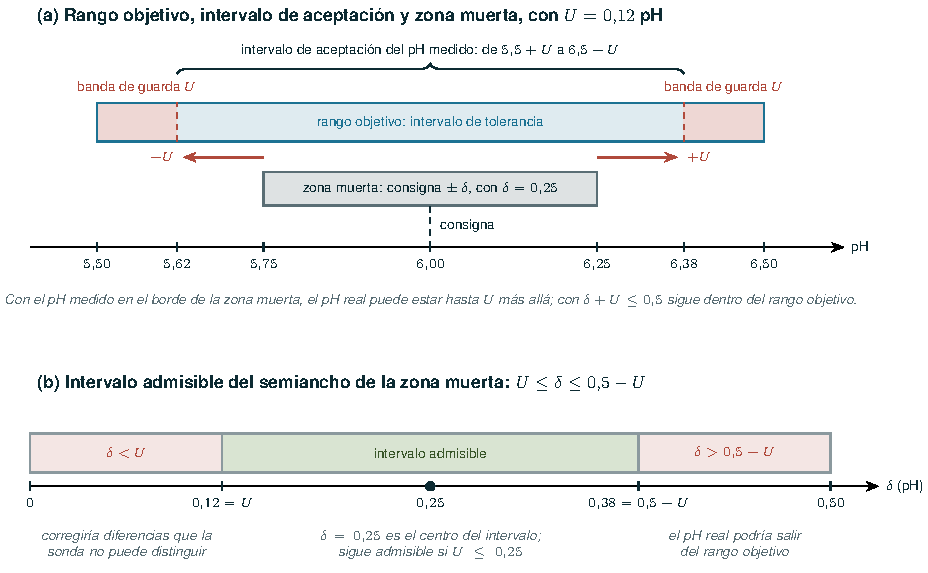
\includegraphics[scale=0.88]{figuras/fig16.pdf}
\caption[Criterio de banda de guarda aplicado a la zona muerta]{Criterio de banda de guarda aplicado a la zona muerta, dibujado a escala con $U=0{,}12$\,pH. (a) Rango objetivo, intervalo de aceptación del pH medido y zona muerta de semiancho $\delta=0{,}25$\,pH: aunque el pH medido quede en el borde de la zona muerta, el real sigue dentro del rango. (b) Intervalo admisible de $\delta$ según la ecuación~\eqref{eq:banda}. Elaborado por los autores (A. Morocho y K. Toledo, TikZ, 2026).}\label{fig:banda}
\end{figure}

La temperatura no se manipula como factor: los ensayos se hacen dentro de una ventana declarada de $22\pm3$\,°C, en la que el error de la compensación es de milésimas de pH (ecuación~\eqref{eq:comp}) y el cambio químico del orden de $\pm0{,}01$\,pH, un orden de magnitud por debajo de $U$. Tampoco se trata como covariable; el intervalo de cada corrida se informa con sus resultados, y el trabajo no puede afirmar el desempeño fuera de la ventana. En cuanto a la concordancia entre resultados, el Vocabulario distingue condiciones de repetibilidad, de precisión intermedia y de reproducibilidad [38]. Con un solo banco no se evalúa la reproducibilidad, sino la repetibilidad dentro de una sesión de calibración y la precisión intermedia entre sesiones; por eso las corridas se reparten en varias sesiones (apartado~\ref{sec:ensayos}).

\subsubsection{Indicadores de dosificación y de productividad}\label{sec:indicadores}
El sistema de dosificación se evalúa con el consumo de ácido y de base y el número de dosis de cada corrida, y con la dosis mínima repetible, su coeficiente de variación y el volumen por revolución al inicio y al final de la campaña, cuya diferencia mide la fatiga del tubo. Estos indicadores miden el desempeño del control, no la productividad del cultivo, que se expresa con el rendimiento por superficie [22], la eficiencia en el uso del agua [30] y el trabajo, del que forma parte la revisión manual del pH [5, 8]. El banco no tiene cultivo, y sus indicadores se relacionan con ellos indirectamente: el tiempo en rango indica cuánto tiempo están disponibles los nutrientes; el consumo se suma a los insumos, y el número de dosis, cuánto interviene el equipo.

\clearpage
\section{Marco Metodológico}\label{sec:mm}

La metodología sigue el orden en que se construye y se evalúa el prototipo (figura~\ref{fig:metodologia}). Primero se fijan los requerimientos de medición y dosificación. Después se diseñan, se construyen y se ponen en marcha la electrónica y el banco. Luego se caracterizan la medición y las bombas, se mide la curva de titulación y se comprueba que la menor dosis no cambie el pH más de la mitad del margen de error; si lo cambia, se diluye más el reactivo. Por último, se diseña el control, se implementa en el firmware y se valida su desempeño.

\begin{figure}[!htb]\centering
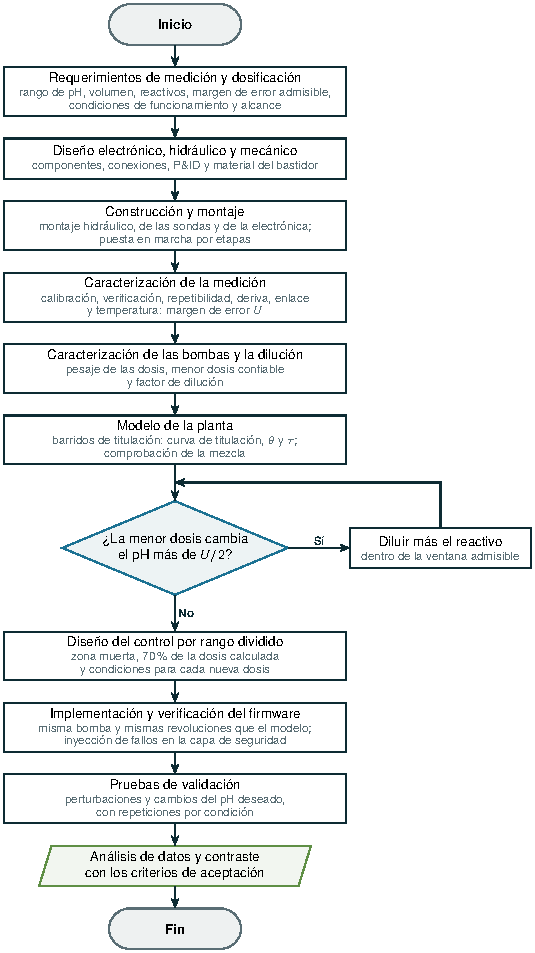
\includegraphics{figuras/fig17.pdf}
\caption[Diagrama de flujo de la metodología]{Diagrama de flujo de la metodología, en el orden de los apartados de este capítulo. El único lazo es el de la regla de dimensionamiento: si la menor dosis cambia el pH más de $U/2$, se diluye más el reactivo y se repite la comprobación. Elaborado por los autores (A. Morocho y K. Toledo, TikZ, 2026).}\label{fig:metodologia}
\end{figure}

% =====================================================================
\subsection{Arquitectura del prototipo}\label{sec:arq}

Antes de construir el prototipo se fija qué debe cumplir. De este apartado sale la tabla de requerimientos, que responde al primer objetivo y es el criterio de aceptación de las caracterizaciones.

\subsubsection{Requerimientos de medición y dosificación}\label{sec:req}
Los requerimientos parten de cinco factores: el rango de pH, el volumen de solución, los reactivos, el margen de error admisible en la medición y las condiciones de funcionamiento. La tabla~\ref{tab:req} da el valor de partida de cada uno y lo que fija, y añade la dosis de las bombas, que es el dato del actuador. La dilución del reactivo es la variable de diseño con la que se cumplen.

\tabla{tab:req}{tab07.pdf}{Requerimientos de medición y dosificación}

La menor dosis se dimensiona con la regla de la ecuación~\eqref{eq:regla}: su efecto sobre el pH, calculado con la ganancia local en cada punto del rango objetivo, no debe superar $U/2$. La regla es una propuesta propia de este trabajo. No procede de una norma ni de los documentos revisados, y se apoya en dos argumentos:
\begin{itemize}
\item Una dosis no debe poder saltar la zona muerta entera. Para eso su efecto debe ser menor que el ancho de esa zona, $2\delta$. Como $\delta\ge U$, basta con que no llegue a $2U$, y el límite $U/2$ deja un margen de cuatro veces.
\item Dosificar en revoluciones enteras redondea el volumen, y ese redondeo se comporta como un error de resolución. Con un paso de pH $q$, su incertidumbre típica es $q/\sqrt{12}$ [39]. Con $q=U/2$ vale 0,29 veces la incertidumbre típica de la medición y, sumada en cuadratura, la aumenta solo un 4\,\%.
\end{itemize}
Con los valores \emph{a priori}, una revolución entrega 0,314\,mL y, con el reactivo diluido 1:10, la ganancia en la consigna es de 0,0554\,pH/mL (tabla~\ref{tab:beta}): esa dosis mueve el pH menos de 0,02 unidades, por debajo de $U/2=0{,}06$\,pH. Según el modelo, la regla es conservadora: con factores de dilución de 1 a 22,8 y zonas muertas de 0,25 y 0,12\,pH, las dos bombas no llegan a alternarse aunque la regla se incumpla. Se trata por eso como un criterio de diseño que debe comprobarse (apartado~\ref{sec:planta}), y no como un límite demostrado.

\subsubsection{Organización del prototipo}\label{sec:org}
El prototipo se organiza en cuatro capas, que reproducen la estructura de un sistema de control de pH industrial a escala de banco: medición, control, actuación y alimentación (figura~\ref{fig:arq}). Se montan sobre un banco hidráulico de reservorio único, que es la planta. Cada requerimiento recae sobre una parte: la incertidumbre, sobre la capa de medición; la dosis mínima repetible, sobre la de actuación y la dilución del reactivo, y la zona muerta, sobre la ley de control que ejecuta el microcontrolador.

\figura{fig:arq}{fig18.pdf}{Arquitectura del prototipo en cuatro capas}{Arquitectura del prototipo en cuatro capas: medición, control, actuación y alimentación. Los distintivos de color indican de qué fuente se alimenta cada elemento; la sonda de pH tiene su propia fuente de 12\,V aislada. Las líneas azules representan el contacto con la solución del depósito T1, cuya disposición hidráulica se describe más adelante. Es un diagrama del diseño propuesto, no del prototipo construido. Elaborado por los autores (A. Morocho y K. Toledo, TikZ, 2026).}

\subsubsection{Alcance y condiciones de funcionamiento}\label{sec:alcance}
El prototipo se evalúa en un depósito de laboratorio, con 10\,L de solución nutritiva de composición declarada, preparada de nuevo para cada sesión, con recirculación y sin plantas. Con un cultivo, la absorción de nutrientes añadiría una perturbación lenta, distinta en cada ensayo, que no puede repetirse ni medirse de forma práctica. Sin él, la perturbación se aplica de forma estandarizada y los resultados pueden atribuirse al controlador. Esos resultados describen el desempeño del control en el banco, no en un cultivo ni en una instalación de producción. Quedan fuera del alcance, como trabajo futuro, el cultivo vegetal y la operación en flujo continuo, el control de la conductividad eléctrica, la telemetría y la optimización del consumo energético. Ninguna de estas exclusiones afecta a los objetivos.

Dentro de ese alcance, el trabajo declara estas limitaciones:
\begin{itemize}
\item Los patrones no tienen certificado de lote, y la incertidumbre no es trazable al SI.
\item La sonda no expone la tensión del electrodo: su pendiente no se mide y se sustituye por el error en el patrón 9,18.
\item Hay un solo banco y tres sesiones de la perturbación principal: se evalúan la repetibilidad y la precisión intermedia, no la reproducibilidad.
\item La perturbación hacia la base y la ley de dosis fija se ensayan en una sola sesión cada una, con dos corridas: sus resultados son descriptivos.
\item Los resultados valen dentro de la ventana de $22\pm3$\,°C.
\end{itemize}

% =====================================================================
\subsection{Diseño electrónico}\label{sec:elec}

La electrónica se define con tres decisiones: qué componentes se usan, cómo se conectan y cómo se alimentan y protegen. El resultado es el esquema de conexiones con que se monta el banco (figura~\ref{fig:esquema}), dentro del segundo objetivo.

\subsubsection{Selección de componentes}
Los componentes se eligen a partir de los requerimientos de la tabla~\ref{tab:req}. La tabla~\ref{tab:componentes} indica, para cada función, qué se utiliza, por qué y qué alternativa se descartó.

\tabla{tab:componentes}{tab08.pdf}{Selección de los componentes}

\subsubsection{Circuitos de medición y de actuación}\label{sec:circuitos}
La sonda de pH se comunica por Modbus RTU sobre RS-485 a 9600 baudios, con 8 bits de datos, sin paridad y un bit de parada, y con la dirección 6 [57]. Se conecta a una USART del microcontrolador a través de un convertidor TTL a RS-485 con aislamiento galvánico, porque el enlace diferencial no aísla por sí mismo. Se alimenta con una fuente de 12\,V dedicada solo a ella, cuya masa no se une a la de los demás rieles, para que la alimentación no puentee el aislamiento del convertidor. La sonda de temperatura DS18B20 se lee por el bus 1-Wire a 12 bits, con una sola resistencia de polarización de 4,7\,k$\Omega$ a 3,3\,V [58]. Antes de la primera medición se comprueba con un polímetro si su vaina metálica está unida a la masa del microcontrolador: si lo estuviera, uniría las masas a través de la solución y habría que cambiar el montaje.

Cada bomba peristáltica se acciona con un controlador TMC2209 en formato \emph{stepstick}, configurado a 1/8 de micropaso con las patillas MS1 y MS2 sin conectar [61]. El microcontrolador le entrega las señales STEP, DIR y de habilitación. Los 24\,V de los controladores pasan por el canal 2 del módulo de relés, que el firmware cierra al arrancar una dosis y abre cuando los dos motores se detienen o cuando entra en fallo. Si el programa se bloquea, el temporizador de vigilancia reinicia la placa, que arranca con los relés abiertos: las bombas quedan sin potencia aunque la señal de habilitación siga activa. El motor de la bomba es de dos fases, 1,2\,A y 20\,W [72]; su corriente se ajusta con el potenciómetro del controlador a unos 0,7\,A ($V_{\text{ref}}\approx1{,}0$\,V), y solo se sube si la bomba pierde pasos. La bomba de recirculación se alimenta del mismo riel a través de un reductor de tensión ajustable, con el que se fija su caudal de trabajo; se enciende y se apaga con el canal 1 del módulo de relés, y un diodo de descarga en sus bornes absorbe el pico de tensión al abrirse el contacto.

\subsubsection{Alimentación, protección y compatibilidad eléctrica}\label{sec:alim}
La alimentación se reparte en tres rieles: uno de 24\,V y al menos 3\,A, para los dos controladores de motor y la recirculación; uno de 5\,V para las bobinas del módulo de relés, conectado a su entrada JD-VCC con el puente retirado, y la fuente aislada de 12\,V de la sonda de pH. La masa del riel de 24\,V y la de la placa se unen en un solo punto; las de 5 y 12\,V no se unen a ella. Cada riel sale de una fuente con protección interna contra sobrecarga y cortocircuito, y el banco se conecta a un tomacorriente protegido por un interruptor diferencial. Para detenerlo por completo se desenchufa: su clavija queda accesible y fuera de la zona húmeda. La electrónica va en un gabinete estanco, con entrada de cables por prensaestopas y separado de los líquidos. La secuencia de operación añade una separación en el tiempo, porque medir, dosificar y esperar evita interrogar a la sonda con las bombas en marcha.

En el riel de 24\,V, el enclavamiento impide que las dos bombas de reactivo trabajen a la vez. El peor caso es una de ellas, de hasta 20\,W, más la recirculación a plena tensión, de 19\,W: unos 1,8\,A, frente a los 5\,A de la fuente disponible. El módulo de relés toma unos 0,16\,A de su fuente de 5\,V, y la sonda de pH, unos 25\,mA [57]. La corriente real de cada riel se mide en la puesta en marcha. La placa toma sus 5\,V del puerto USB del computador, por el que también salen los datos. En las corridas, el computador trabaja con su batería, para no introducir por el USB la tierra de la red; los barridos de titulación duran más que esa batería, y la tasa de tramas erróneas que el firmware anota en cada punto muestra si esa conexión afecta al enlace.

Los niveles de cada conexión son compatibles: las salidas de la placa son de 3,3\,V, y tanto el controlador de motor [61] como el lado lógico del convertidor RS-485 admiten lógica de 3,3 a 5\,V; el DS18B20 admite de 3,0 a 5,5\,V [58], y la sonda de pH, de 12 a 24\,V [57]. Las entradas del módulo de relés son activas por nivel bajo, y sus contactos están marcados para 10\,A a 30\,V de continua. La figura~\ref{fig:esquema} reúne las conexiones, con el pin de la placa que usa cada señal.

\figura{fig:esquema}{fig19.pdf}{Esquema de conexiones eléctricas del prototipo}{Esquema de conexiones eléctricas del prototipo. Los símbolos de riel (+24V, +3V3, GND y los demás) indican a qué alimentación va cada pin, en lugar de dibujar todos los cables, y entre paréntesis se indica la serigrafía del pin en la placa. Es un esquema del diseño propuesto, no del prototipo construido. Elaborado por los autores (A. Morocho y K. Toledo, KiCad, 2026).}

% =====================================================================
\subsection{Diseño hidráulico y mecánico del banco}\label{sec:hid}

El banco es donde se ensaya el control. Su diseño fija los depósitos, el recorrido de cada líquido, la posición de las sondas y el bastidor que lo sostiene (figura~\ref{fig:pid}).

\subsubsection{Arquitectura hidráulica}\label{sec:archid}
El banco es una torre de reservorio único, con tres depósitos. T1 contiene la solución de trabajo: 10\,L útiles, marcados sobre un recipiente de 12 a 15\,L; aloja la sonda de pH, la de temperatura y la aspiración de la recirculación, y es el objeto de control. T3 y T4, de 2\,L cada uno, contienen el ácido y la base diluidos, sobre una bandeja de contención de al menos 5\,L; el venteo de T4 lleva cal sodada, para que el KOH no absorba CO$_2$ del aire. No hay depósito de reposición: reponer agua durante la corrida cambiaría a la vez el volumen, la alcalinidad y la capacidad tampón, y el consumo observado no podría atribuirse a la acción de control.

Cada sesión parte de un lote fresco, que se prepara a mano en T1. Se pone agua de red por debajo de la marca, se añaden las soluciones A, B y C por separado con la recirculación en marcha, y se enrasa a 10\,L: con un solo recipiente, el orden de adición es la única barrera frente a la precipitación. La descarga de la recirculación cae al aire sobre la superficie de T1, de modo que el sistema es abierto al CO$_2$ por decisión de diseño. Con el retorno sumergido, la solución conservaría la capacidad tampón del carbonato del agua de red: corregir la perturbación de los ensayos exigiría unos 253\,mL de reactivo en lugar de 30, según el modelo, y el límite de volumen acumulado abortaría corridas legítimas. A cambio, cada lote necesita un pre-despojo, para que el CO$_2$ escape antes de la corrida: se acidifica el lote a la consigna, se recircula sin dosificar hasta que el pH alcanza una meseta, y se reajusta a la consigna hasta que el pH se mantiene estable. Sin acidificar, la recirculación solo retiraría el CO$_2$ en exceso, y el bicarbonato permanecería en el lote.

\figura{fig:pid}{fig20.pdf}{Diagrama P\&ID del banco}{Diagrama P\&ID del banco. Las líneas continuas son de proceso, y las discontinuas, de señal. T3 y T4 quedan por debajo del nivel de líquido de T1, y el reactivo gotea en el chorro de retorno desde un hueco de aire. No está a escala; es un diagrama del diseño propuesto, no del prototipo construido. Elaborado por los autores (A. Morocho y K. Toledo, TikZ, 2026).}

\subsubsection{Elementos de diseño y mantenimiento}\label{sec:elementos}
El reactivo se dosifica por goteo dentro del chorro de retorno de la recirculación, que lo dispersa antes de que alcance el electrodo. Las puntas de los tubos quedan fijas uno o dos centímetros por encima de la boca de la manguera: ese hueco de aire rompe el sifón en las dos descargas, y además T3 y T4 se sitúan por debajo del nivel de líquido de T1. El volumen de partida se fija contra la marca de 10\,L, que se verifica y se anota en la bitácora antes del pre-despojo, junto con todo lo que se añade al lote después. La marca no detecta fugas durante la corrida, a diferencia de un sensor de nivel: al final de cada corrida se inspecciona el banco. Una válvula de vaciado en el fondo de T1, su única perforación bajo el nivel de líquido, permite preparar el lote siguiente.

La sonda de pH se monta en T1, nunca en la línea de recirculación, donde vería el bolo sin mezclar. Va sujeta al bastidor, sumergida un tercio de su longitud (unos 62\,mm de 185) e inclinada al menos 15° respecto de la horizontal, con la punta hacia abajo, como indica el fabricante [57]; el tramo que la sostiene tiene tres profundidades marcadas. Se retira hacia arriba sin vaciar T1, para calibrarla y guardarla con la punta en cloruro de potasio de 3,5\,mol/L. El cabezal de cada bomba queda accesible para cambiar el tubo, y cambiar la punta o la altura de descarga obliga a repetir la gravimetría. Con los depósitos llenos, las bombas y el gabinete, el bastidor soporta unos 20\,kg.

\subsubsection{Selección del material del bastidor}\label{sec:bastidor}
El material se elige con el método de Ashby (apartado~\ref{sec:materiales}). La función del bastidor es sostener los depósitos, las bombas, las sondas y el gabinete, y fijar sus alturas relativas. Las restricciones son tres: la flecha de los travesaños debe ser menor que 1\,mm bajo la carga, muy por debajo de la holgura de las puntas de goteo; el material debe resistir las salpicaduras de los reactivos de hasta 1\,N, y el bastidor debe armarse con herramientas de mano. El objetivo es el costo mínimo, y las variables libres, el material y la sección comercial. El filtrado por resistencia química (tabla~\ref{tab:compat}) descarta el aluminio y el acero inoxidable 304, y la tabla~\ref{tab:candidatos} ordena los tres candidatos que pasan por el índice de una viga rígida y ligera, $E^{1/2}/\rho$.

\tabla{tab:candidatos}{tab09.pdf}{Candidatos que pasan el filtrado y su índice de material}

En el banco, sin embargo, la rigidez no limita. Un travesaño de tubo de PVC de presión de 1 pulgada, de 33,40\,mm de diámetro exterior y 4,55\,mm de espesor [76], tiene un momento de inercia $I=\pi(D^4-d^4)/64\approx44\,000$\,mm$^4$. Con 40\,cm entre apoyos y la mitad del peso de T1 lleno, unos 59\,N, aplicada en el centro, se flecta
\begin{equation}
\delta=\frac{F\,L^3}{48\,E\,I}\approx0{,}65\ \text{mm}\label{eq:flecha}
\end{equation}
con $E=2{,}76$\,GPa, por debajo del milímetro de la restricción. Como el material peor clasificado ya cumple con holgura, deciden el objetivo y la documentación: el PVC rígido de presión se fabrica en el país con una amplia gama de accesorios, se corta con sierra y se rosca a mano [76], mientras que el polipropileno de la ficha consultada es un semielaborado para tanques y equipos [74]. El bastidor se arma con tubo y accesorios de PVC rígido de presión de 1 pulgada; los recipientes son de polietileno o de polipropileno, y la bandeja de contención, de polipropileno o de PVC [69]. La luz de 40\,cm es una hipótesis de partida, y la flecha se recalcula con las medidas del bastidor armado.

% =====================================================================
\subsection{Construcción y montaje}\label{sec:mont}

El banco se monta y después se pone en marcha por etapas, para que un fallo quede acotado a lo último que se conectó. El montaje sigue este orden:
\begin{enumerate}
\item Depósito T1. Es un recipiente de grado alimentario, de boca ancha y paredes rectas, con la marca de 10\,L. La válvula de vaciado se monta en el fondo con un pasamuros estanco, y la descarga de la recirculación se fija sobre la superficie.
\item Depósitos de reactivo. T3 y T4 son botellas de HDPE o polipropileno con tapa perforada para el tubo y venteo, colocadas sobre la bandeja de contención. La base diluida se prepara por lotes, con la fecha registrada.
\item Líneas de dosificación. Cada bomba tiene un tubo de 3,2\,mm de diámetro interior, con un lastre con malla en la succión, hasta el soporte de goteo, que fija las dos puntas, cortadas en bisel, sobre la boca de la manguera de retorno.
\item Sondas. La de pH y la de temperatura se sujetan al bastidor, sumergidas en T1 y lejos del chorro de retorno.
\item Electrónica. En el gabinete se montan la placa, los dos controladores de motor sobre una placa perforada con borneras, el módulo de relés, el reductor, el convertidor RS-485 y las fuentes, según el esquema de la figura~\ref{fig:esquema}. Antes de energizar se comprueba la continuidad de cada conexión y que la masa de la sonda de pH quede aislada del resto.
\end{enumerate}
Cada etapa de la puesta en marcha tiene una prueba que debe superarse antes de pasar a la siguiente:
\begin{enumerate}
\item La placa sola, conectada por USB: enciende y el computador la reconoce.
\item El proyecto del firmware en STM32CubeIDE: compila sin errores.
\item La placa grabada: la consola serie responde y el pulsador B1 se registra.
\item El módulo de relés sin cargas: se confirma con qué nivel se activa cada canal y que arranca con los contactos abiertos.
\item La sonda de pH: se lee por Modbus desde la consola, y también la sonda de temperatura.
\item Las bombas dosificadoras: con los comandos de prueba y el límite de corriente ajustado, se comprueba el sentido de giro y que una revolución entrega unos 0,314\,mL.
\item La bomba de recirculación: se fija la tensión del reductor y se comprueba que el relé la enciende y la apaga.
\end{enumerate}
Con todo conectado, se mide la corriente de cada riel y, con las bombas detenidas, se comprueba que no haya fugas ni sifonamiento.

% =====================================================================
\subsection{Caracterización de la medición}\label{sec:carmed}

El margen de error de la medición del pH se expresa como una incertidumbre expandida $U$, con factor de cobertura $k=2$, según la GUM [39]. Se obtiene con estos ensayos, que se hacen con la sonda en los patrones de la serie GB:
\begin{enumerate}
\item Calibración. Al inicio de cada sesión, la sonda se calibra en dos puntos, con el cero en 6,86 y la pendiente en 4,00, según el procedimiento del fabricante [57]. Los patrones en polvo se reconstituyen en alícuotas de 250\,mL, con agua destilada recién abierta.
\item Verificación independiente. Se lee el patrón 9,18, que nunca entra en la calibración, y la lectura se compara con su valor tabulado a la temperatura registrada. La diferencia es el error de verificación.
\item Repetibilidad. En cada patrón se toman diez lecturas independientes, retirando y volviendo a sumergir la sonda, y se calcula su desviación típica.
\item Deriva. Se registra la lectura sobre el patrón 4,00 durante 2\,h; la pendiente de ese registro no debe superar 0,02\,pH/h. Se usa el 4,00 porque el patrón alcalino absorbe CO$_2$ del aire.
\item Enlace de medición. El firmware cuenta los errores de trama Modbus y anota su tasa en cada medición, con la recirculación parada y en marcha. La tasa no debe superar el 1\,\%, y ningún fallo consecutivo debe impedir completar una decisión. Se compara además, una vez, la lectura media con la bomba en marcha y parada.
\item Temperatura. La temperatura interna que la sonda reporta por Modbus se compara en todos los ensayos con la del DS18B20. Una diferencia sostenida mayor que $\pm0{,}5$\,°C indicaría que la compensación trabaja con una temperatura errónea.
\end{enumerate}
Con esos resultados se construye el presupuesto de incertidumbre, aplicando la ecuación~\eqref{eq:gum}. La repetibilidad entra como contribución de tipo A; el error de verificación, que acota el sesgo de la calibración, la tolerancia del patrón y la resolución, como contribuciones de tipo B, y la compensación térmica, como una contribución acotada por la ventana de temperatura. El resultado se presenta como en la tabla~\ref{tab:presupuesto-u} y se acepta si $U\le0{,}15$\,pH; si resulta mayor, se procede como indica el apartado~\ref{sec:incertidumbre}. La deriva no entra en la suma: se contrasta con su criterio. La dinámica de la sonda no se ensaya por separado, porque queda incluida en la del conjunto tanque-electrodo (apartado~\ref{sec:planta}).

% =====================================================================
\subsection{Caracterización de las bombas y la dilución}\label{sec:carbom}

Aquí se determina cuánto entrega cada bomba por revolución y cuál es su menor dosis confiable, y con esos datos se elige la dilución del reactivo. Todo se mide pesando lo que entrega la bomba:
\begin{enumerate}
\item Gravimetría. Con el tubo, la altura de descarga y la contrapresión fijos y documentados, se pesan 5 niveles de volumen, con 5 repeticiones por nivel y por bomba, en una balanza de 0,01\,g. La pendiente de la recta entre el volumen pesado y las revoluciones es el volumen por revolución, y la relación se acepta como lineal si $R^2\ge0{,}99$. El punto central se repite al inicio y al final de la campaña, para vigilar la fatiga del tubo.
\item Dosis mínima repetible. Se baja el número de revoluciones nivel a nivel, con 10 pesadas en cada uno, y se calcula el coeficiente de variación una vez descontada la varianza de la balanza: $\sigma^2_{\text{bomba}}=\sigma^2_{\text{medida}}-\sigma^2_{\text{balanza}}$. La dosis mínima repetible es el menor número entero de revoluciones con un coeficiente no superior al 5\,\%.
\item Factor de dilución. Se multiplica la dosis mínima repetible por la ganancia local máxima dentro del rango objetivo, y se elige la dilución para que el producto no supere $U/2$ (ecuación~\eqref{eq:regla}).
\end{enumerate}
La tabla~\ref{tab:regla} hace ese cálculo antes de los ensayos, con los parámetros \emph{a priori}. Sin diluir, una dosis mínima movería 0,21\,pH en la consigna, 3,5 veces más que $U/2$. La regla se exige en todo el rango objetivo, donde manda el punto de mayor ganancia, pH 5,5, que pide $D\ge7{,}7$.

\tabla{tab:regla}{tab10.pdf}{Evaluación a priori de la regla de dimensionamiento, con $\Vmin=0{,}314$\,mL y $U=0{,}12$\,pH}

La dilución tiene también un límite superior: se impone que la mayor corrección prevista, de una unidad de pH, no añada más del 1\,\% del volumen del depósito. Con $D=10$ exige 43,8\,mL, según la curva del modelo, y de ahí resulta $D\le22{,}8$. La ventana admisible es $7{,}7\le D\le22{,}8$, y la dilución de partida, de 1:10, queda dentro. La ventana se cierra si la dosis mínima repetible medida supera 0,93\,mL, es decir, tres revoluciones o más.

% =====================================================================
\subsection{Modelo de la planta}\label{sec:planta}

La planta se describe primero con el modelo del proceso en MATLAB, abierto al CO$_2$, del que salen la curva de titulación y los parámetros \emph{a priori} con que se dimensionan el banco y el control. Los ensayos de este apartado sustituyen esos valores por los medidos, dentro del tercer objetivo.

\subsubsection{Curva y ganancia que predice el modelo}
En la solución de este trabajo, con 1,3\,mM de fosfato y el carbonato en equilibrio con el aire, $\beta$ vale $1{,}81\cdot10^{-4}$\,eq/(L·pH) en la consigna, casi todo por el fosfato. La figura~\ref{fig:titulacion} muestra la curva de titulación que predice la ecuación~\eqref{eq:electro} para un lote de 10\,L tras el pre-despojo, con ácido sulfúrico diluido a 0,1\,N: es casi lineal y tendida por encima de la consigna, y muy empinada por debajo de 5,5. La tabla~\ref{tab:beta} da la capacidad tampón y la ganancia local de la ecuación~\eqref{eq:kp}: la ganancia cambia unas 15 veces entre pH 5,0 y 7,0, y 3,5 veces entre la consigna y pH 6,8.

\figura{fig:titulacion}{fig21.pdf}{Curva de titulación y ganancia local predichas por el modelo}{Curva de titulación y ganancia local del proceso predichas por el modelo para 10\,L de solución nutritiva tras el pre-despojo, con ácido sulfúrico 0,1\,N. (a) pH frente al volumen de ácido añadido, con el rango objetivo sombreado. (b) Ganancia local $K_p=|d\mathrm{pH}/dV|$ frente al pH, en escala logarítmica. Parámetros \emph{a priori}; la curva real se mide al caracterizar la planta. Elaborado por los autores (A. Morocho y K. Toledo, MATLAB, 2026).}

\tabla{tab:beta}{tab11.pdf}{Capacidad tampón y ganancia local del proceso predichas por el modelo}

\subsubsection{Curva de titulación}\label{sec:barridos}
La curva que se graba en el firmware se mide con dos barridos completos de ida y vuelta, cada uno sobre un lote fresco. El lote se lleva a pH 7,1 y se titula hacia abajo con ácido hasta pH 5,0; sin cambiar de lote, se titula hacia arriba con base hasta 7,0. Tras cada dosis se espera al menos $5\tau+\theta$. Cada bomba cubre así el rango de caracterización, de 5,0 a 7,0, que contiene el tramo en que trabaja el control, de 5,4 a 6,8. Antes de los barridos se hace un ensayo piloto de titulación, sobre un lote propio, en el que se comprueban la mezcla, que el reactivo calculado con la curva coincide con el que hace falta y el criterio de ajuste del modelo dinámico.

Cada dosis se dimensiona para mover el pH unas 0,10 unidades: el controlador interpola el volumen acumulado, y el error de esa tabla lo fija el ruido de la lectura, no el paso. Un barrido tiene 42 dosis y dura unas 8,6\,h, de modo que cabe en una jornada de laboratorio. Los barridos son automáticos, con la capa de seguridad activa, y se detienen si la temperatura sale de la ventana. Hay tres pausas de 30 minutos sin dosificar (al empezar, al cambiar de rama y al terminar), que miden la deriva de la sonda junto con la desgasificación, que se descuenta de la curva. La ganancia local se estima por regresión local centrada, con la misma ventana de $\pm0{,}15$\,pH en las dos ramas, y la curva que se graba es la media de los dos barridos. La razón entre las ganancias de las dos bombas cerca de la consigna se informa de forma descriptiva.

\subsubsection{Dinámica e identificación}\label{sec:ident}
No se hacen ensayos de escalón aparte: cada dosis de la titulación es una entrada de volumen conocido, y su respuesta, registrada cada 10\,s durante la espera, basta para ajustar el modelo de la ecuación~\eqref{eq:fopdt}. El ajuste toma como entrada el caudal de la bomba durante la duración registrada de la dosis, y es conjunto: un mismo $\theta$ y un mismo $\tau$ por bomba para todas las dosis de un barrido. Esas lecturas se toman con la recirculación en marcha, porque apagarla cambiaría la mezcla que se quiere identificar; la lectura que decide la dosis siguiente se toma con ella apagada, como en las corridas. El modelo se ajusta con las dosis de un barrido y se valida con las del otro: se acepta si el índice de la ecuación~\eqref{eq:fit} llega al 80\,\% sobre el barrido de validación y los residuos tienen media próxima a cero y no presentan estructura.

Con los dos parámetros se fija la espera entre dosis, $\theta+3\tau$. Con los valores \emph{a priori} de la cascada, 15\,s de retardo de transporte y $90+13$\,s de constantes de mezcla y de electrodo, resultan unos 324\,s, el valor fijado en el firmware; con el primer orden identificado sobre ella, de 27,6 y 98,0\,s, 322\,s. Al cabo de ese tiempo la respuesta ha recorrido el 96\,\% de su valor final (figura~\ref{fig:respuesta}), y con $\theta+5\tau$, el 99,6\,\%.

\figura{fig:respuesta}{fig22.pdf}{Respuesta normalizada a una dosis según el modelo del banco}{Respuesta normalizada a una dosis según el modelo del banco: cascada de transporte (15\,s), mezcla (90\,s) y electrodo (13\,s), frente al primer orden con retardo identificado sobre ella ($\theta=27{,}6$\,s, $\tau=98{,}0$\,s), con los puntos del 28,3 y el 63,2\,\% del método de dos puntos. La línea vertical marca el periodo de decisión, al que la cascada ha recorrido el 96\,\% de su valor final. Parámetros \emph{a priori}. Elaborado por los autores (A. Morocho y K. Toledo, MATLAB, 2026).}

\subsubsection{Comprobación de la mezcla y de la regla de dimensionamiento}\label{sec:comprobacion}
Cada medición solo vale si la solución está mezclada cuando se lee. En el ensayo piloto se aplica tres veces la misma dosis de ácido con la sonda en cada una de sus tres profundidades marcadas. La mezcla se considera adecuada si el cambio final de pH coincide en las tres profundidades dentro de $U$ y si, al cumplirse la espera, la lectura ha recorrido al menos el 95\,\% de ese cambio; si no, se alarga la espera o se aumenta el caudal de recirculación antes de la campaña.

La regla de la ecuación~\eqref{eq:regla} se comprueba de dos formas. Con los valores medidos: se multiplica la dosis mínima repetible por la ganancia local de la curva en cada punto del rango objetivo, y el producto se compara con $U/2$; si lo supera, se diluye más el reactivo dentro de la ventana admisible y se repite la comprobación. Y en los ensayos de validación: las dos bombas no deben alternarse en ninguna corrida, y el pH alcanzado tras cada dosis debe coincidir, dentro de $U$, con el que predice la curva.

% =====================================================================
\subsection{Diseño del control}\label{sec:control}

El control es el de demanda de reactivo con rango dividido y zona muerta (apartado~\ref{sec:demanda}). Aquí se fijan sus parámetros, se describe el ciclo que ejecuta el firmware y se da la predicción que sirve de referencia a la validación.

\subsubsection{Zona muerta y ciclo de control}\label{sec:ciclo}
La zona muerta se fija en $\delta=0{,}25$\,pH a cada lado de la consigna, el centro del intervalo admisible de la ecuación~\eqref{eq:banda} [51]. Ese valor es admisible para cualquier $U\le0{,}25$, y puede declararse antes de caracterizar la medición. La figura~\ref{fig:ciclo} muestra el ciclo que el firmware repite durante la corrida:
\begin{enumerate}
\item Inicio. El operador arranca la corrida con una pulsación larga del pulsador B1, después de inyectar el bolo o de cambiar la consigna.
\item Asentamiento. La recirculación queda en marcha durante la espera $\theta+3\tau$.
\item Lectura. El firmware apaga la recirculación y lee el pH y la temperatura. Sin una lectura válida no decide ni dosifica, y si pasa un minuto seguido sin ella pasa al estado de fallo (S4).
\item Efecto de la dosis anterior. Si en el ciclo anterior hubo una dosis, suma su volumen al acumulado de esa bomba y compara el cambio de pH que produjo con el que predice la curva (S5).
\item Fallos. Si la lectura está fuera del rango físico o se queda estática dentro de la zona muerta (S4), o si la dosis anterior no tuvo efecto (S5), pasa al estado de fallo y detiene las bombas.
\item Zona muerta. Si $|e|\le\delta$, con $e=\pHm{medido}-\pHm{consigna}$, no se dosifica: se espera otro periodo con la recirculación apagada. Cuando el pH lleva 30 minutos seguidos dentro de la zona muerta, se registra el fin de la corrida.
\item Elección de la bomba y cálculo del volumen. Fuera de la zona muerta actúa la bomba de ácido si $e>\delta$ y la de base si $e<-\delta$, nunca las dos a la vez, con el volumen de la ecuación~\eqref{eq:vcmd} y $\gamma=0{,}70$. Por ejemplo, tras el bolo de los ensayos el pH medido es 6,80; la curva del modelo indica 30,4\,mL de ácido hasta la consigna, y el 70\,\% son 21,3\,mL si $\klote=1$.
\item Redondeo. El volumen se pasa a revoluciones completas: 21,3\,mL son 68 revoluciones. Si lo calculado no llega a media revolución, no se dosifica.
\item Límite acumulado. Si esa bomba ha dosificado más de 250\,mL en la última hora (S2), el firmware pasa al estado de fallo.
\item Dosificación. La bomba gira las revoluciones calculadas, con la recirculación en marcha y solo si la otra bomba está detenida, y el ciclo vuelve al asentamiento.
\end{enumerate}
Si una dosis dejara el pH al otro lado de la zona muerta, actuaría la bomba contraria con las mismas condiciones. Ese caso se registra, porque es el comportamiento que se quiere evitar.

\begin{figure}[!htb]\centering
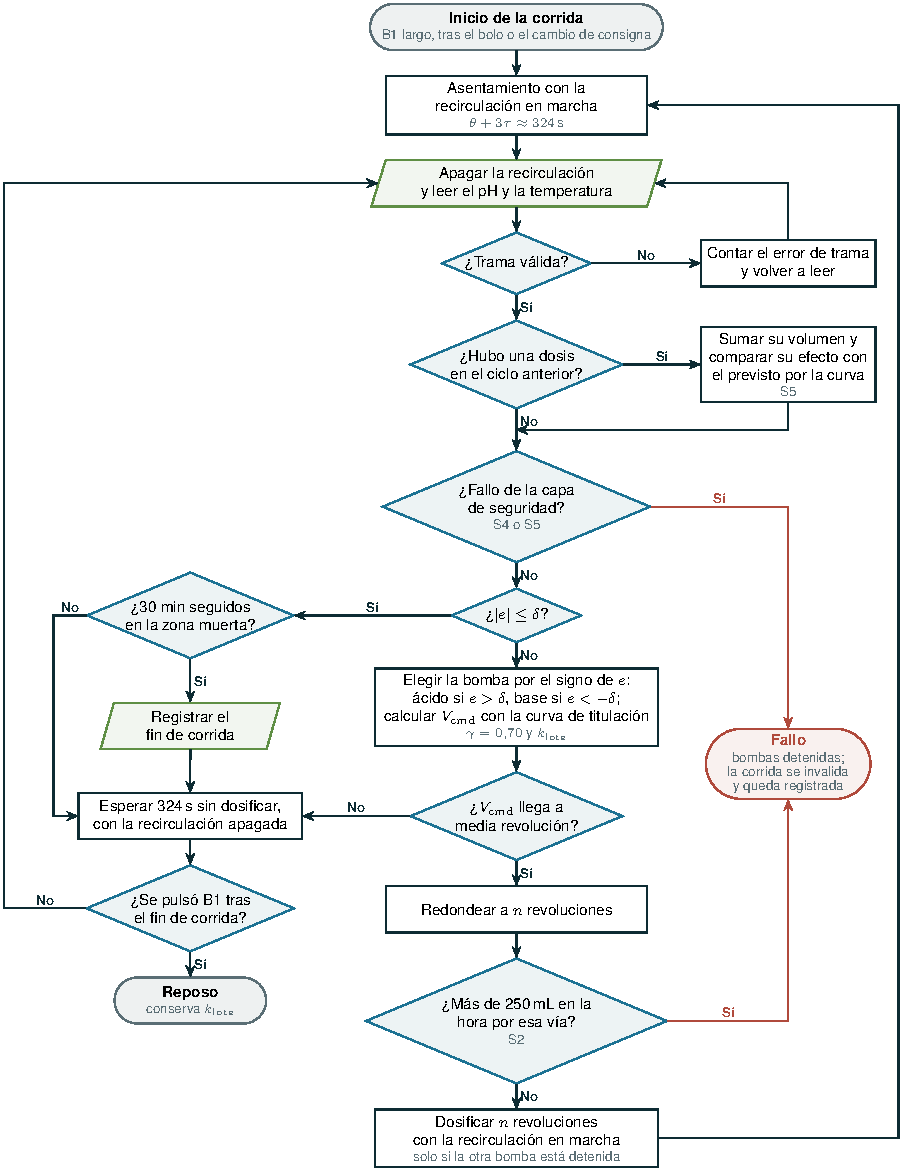
\includegraphics{figuras/fig23.pdf}
\caption[Diagrama de flujo del ciclo de control durante la corrida]{Diagrama de flujo del ciclo de control durante la corrida, en el orden en que el firmware hace las comprobaciones. El error $e$ es el pH medido menos la consigna, y $V_{\text{cmd}}$, el volumen de la ecuación~\eqref{eq:vcmd}. S2, S4 y S5 son mecanismos de la capa de seguridad (tabla~\ref{tab:seguridad}). Se omiten la autocalibración del lote y el modo de barrido. Elaborado por los autores (A. Morocho y K. Toledo, TikZ, 2026).}\label{fig:ciclo}
\end{figure}

\subsubsection{Autocalibración de la curva y protección frente a una corrección excesiva}\label{sec:autocal}
La curva se mide sobre unos lotes y se usa sobre otros, que pueden tener algo más o algo menos de fosfato. Por eso se reajusta al preparar cada lote: el reajuste a la consigna tras el pre-despojo lo hace la bomba de ácido con un volumen conocido $V_{\text{cal}}$, y se mide el pH antes y después, ya asentado. El factor que reescala la curva es
\begin{equation}
\klote=\frac{\sum V_{\text{cal}}}{\sum\bigl(\bigl|\mathcal V(\pHm{antes})-\mathcal V(\pHm{después})\bigr|+\Delta V_{\text{carb}}\bigr)}\label{eq:klote}
\end{equation}
El término $\Delta V_{\text{carb}}$ descuenta el ácido que consume el bicarbonato en equilibrio con el aire al bajar de la meseta del despojo a la consigna; sin él, el factor saldría sesgado al alza entre un 3,6 y un 6,4\,\%. La calibración recorre casi el mismo tramo de pH que el control, así que el sesgo de la sonda se cancela en buena parte. Con la bomba de ácido se cancela también el error sistemático del volumen por revolución, pero no con la de base, y el modelo prevé un error de dosis de alrededor del 3\,\%.

Una dosis excesiva solo podría compensarse con el reactivo contrario, y el control lo evita de cuatro formas: aplica el 70\,\% de lo calculado, reajusta la curva en cada lote, no extrapola la curva fuera del rango en que se midió y acota con el límite acumulado lo que puede dosificarse en una hora. La fracción de 0,70 se eligió comparándola en el modelo con la dosis completa, que ahorra unos 5 minutos por corrida pero cruza la zona muerta mucho más a menudo si falla el reajuste del lote. Si en el ensayo piloto la cantidad calculada difiere en más de un 5\,\% de la que hizo falta, la fracción se reduce.

\subsubsection{Simulación}\label{sec:simulacion}
Antes de implementarlo, el control se simula en MATLAB sobre el modelo del proceso. Con los parámetros \emph{a priori}, corrige la perturbación de los ensayos con dos dosis y unos 28\,mL de ácido; los demás valores esperados están en la tabla~\ref{tab:criterios}. La figura~\ref{fig:leyes} compara la ley por demanda con una de ganancia fija, sintonizada con la ganancia de la consigna y con $\gamma=1$: a pH 6,8, la ganancia fija pide 14,4\,mL donde la curva indica 30,4\,mL. Según el modelo, un PID sintonizado así necesitaría de tres a cuatro dosis para corregir esa perturbación, frente a las dos del control propuesto.

\figura{fig:leyes}{fig24.pdf}{Volumen que pide cada ley de control en función del pH medido}{Volumen que pide cada ley de control en función del pH medido, con la zona muerta de semiancho 0,25\,pH. La ley por demanda lee de la curva de titulación el volumen hasta la consigna y aplica el 70\,\% de esa demanda; la ganancia fija divide el error por la ganancia de la consigna. Por encima de la consigna, en la región tamponada por el fosfato, la ganancia fija pide bastante menos de lo necesario; por debajo, bastante más. Parámetros \emph{a priori}. Elaborado por los autores (A. Morocho y K. Toledo, MATLAB, 2026).}

% =====================================================================
\subsection{Implementación en el firmware}\label{sec:fw}

El control se implementa en la placa y se verifica que el firmware decide lo mismo que el modelo. Los resultados son el firmware verificado y la capa de seguridad probada, con los que se completa el tercer objetivo.

\subsubsection{Estructura del firmware y secuencia de operación}\label{sec:estructura}
El firmware se escribe en C con STM32CubeIDE para la placa Nucleo-G474RE, sin sistema operativo, como un bucle principal con la máquina de estados de la figura~\ref{fig:estados}. La ley de control, la capa de seguridad y la autocalibración del lote se escriben como funciones puras, sin la capa de abstracción del fabricante, y pueden verificarse fuera de la placa. La curva de titulación entra como una tabla generada desde el modelo en MATLAB, que se regenera con la curva medida antes de la campaña. Los demás parámetros se fijan al compilar, a partir de las caracterizaciones, y no cambian durante una corrida; solo cambian entre corridas el factor $\klote$ y la consigna de los escalones, que el operador elige por la consola, lo mismo que la ley de dosis fija de las corridas de referencia.

El prototipo opera por lotes. La preparación del lote y el pre-despojo son manuales y supervisados; la autocalibración reajusta el lote a la consigna y calcula $\klote$, y la corrida es autónoma hasta que el pH lleva 30 minutos seguidos dentro de la zona muerta. Los estados del firmware son el reposo, los de la corrida, los tres equivalentes de la autocalibración y el de fallo, que es terminal: las bombas quedan detenidas y solo se sale de él reiniciando la corrida tras diagnosticar la causa, de modo que un fallo invalida la corrida y queda registrado.

Los fallos se declaran durante la corrida. En cada medición, el firmware comprueba el efecto de la dosis anterior, la lectura nueva y el volumen acumulado, y si la capa de seguridad detecta un fallo pasa al estado de fallo y detiene las bombas. En la autocalibración no se declaran fallos, aunque el enclavamiento de las bombas y el temporizador de vigilancia siguen activos.

\figura{fig:estados}{fig25.pdf}{Estados del firmware y eventos que llevan de uno a otro}{Estados del firmware y eventos que llevan de uno a otro. Una pulsación corta del pulsador B1 lanza una pasada de autocalibración del lote, que vuelve al reposo con el factor $\klote$, o sin dosificar si el lote ya está en la consigna; una pulsación larga arranca la corrida tras el bolo de perturbación o el cambio de consigna, y otra, tras el fin de corrida, vuelve al reposo. Los tiempos son los fijados en el firmware. Se omiten las órdenes de la consola en el reposo. Elaborado por los autores (A. Morocho y K. Toledo, TikZ, 2026).}

\subsubsection{Interfaz, registro y almacenamiento de datos}\label{sec:registro}
La interfaz con el operador es mínima: el pulsador de la placa arranca las fases que requieren una decisión humana, y las variables se visualizan y se registran por una consola serie, a través del puerto serie virtual del depurador. Se registran:
\begin{itemize}
\item En cada medición, el pH, la temperatura del DS18B20, la temperatura interna de la sonda, el tiempo de la corrida y la tasa de tramas erróneas.
\item En cada dosis, la vía y el número de revoluciones, con los volúmenes acumulados de cada reactivo.
\item Cada cambio de estado o fallo, con su causa.
\end{itemize}
Ese registro, capturado en un computador, es la fuente de datos de los ensayos. La consola es también la única señalización, porque el prototipo no lleva indicadores luminosos ni sonoros.

Un programa de terminal en el computador, PuTTY, guarda en un archivo de texto todo lo que la consola imprime. Ese archivo es el dato bruto, y se trata con los criterios habituales de integridad de los datos [53]: se identifica por su fecha, su lote y su sesión, se conserva sin modificar y se respalda en un segundo soporte al terminar cada sesión, junto con la bitácora de preparación del lote. Una lectura perdida queda registrada como tal, y una corrida invalidada se conserva con su causa. Los resultados se calculan con programas de análisis a partir de los archivos originales, de modo que el cálculo puede repetirse.

\subsubsection{Verificación del firmware}\label{sec:verif}
La ley de control se verifica contra el modelo antes de usarla en el banco. Un programa reproduce el código que se compila, con la misma aritmética de coma flotante de 32 bits, y compara sus decisiones con las de los controladores del modelo sobre una misma secuencia de lecturas: se aprueba si coinciden la bomba elegida y el número de revoluciones en todas ellas. En el banco, cada etapa de la puesta en marcha prueba los periféricos que conecta, y durante los ensayos el firmware registra el instante de cada decisión con el reloj real de la corrida. Para la titulación hay un modo de barrido automático, cuya secuencia se contrasta también con la del modelo: deben coincidir las ramas, las pausas y el número de dosis, y las revoluciones de cada dosis no deben diferir en más de una.

\subsubsection{Capa de seguridad}\label{sec:seg}
Sobre la ley de control se superpone una capa de seguridad independiente de ella, porque el banco dosifica sustancias corrosivas con actuadores de 24\,V junto a un volumen de líquido. La tabla~\ref{tab:seguridad} resume sus mecanismos; todos se verifican por inyección deliberada de fallos, con el criterio de detectar el 100\,\% de los fallos inyectados.

\tabla{tab:seguridad}{tab12.pdf}{Mecanismos de la capa de seguridad}

Dos salvaguardas son delicadas de dimensionar, por la ganancia variable del proceso. El límite de volumen acumulado (S2) debe quedar por encima de la máxima demanda legítima que predice la curva, o abortaría corridas válidas. La detección de dosificación sin efecto (S5) no puede exigir que cada dosis desplace el pH por encima de un umbral fijo, porque en la región tamponada una dosis correcta no lo alcanza. Por eso S5 acumula el desplazamiento esperado según la curva,
\begin{equation}
\text{esperado}=\sum_i V_i\left|\frac{d\mathrm{pH}}{dV}\right|_{\text{curva}}(\mathrm{pH}_i)\label{eq:esperado}
\end{equation}
y solo emite juicio cuando ese esperado supera $U/2$: si entonces el desplazamiento observado no llega a la mitad del esperado, declara el fallo. En la comprobación del firmware frente al modelo, sin hardware, no hubo falsas alarmas en 18 corridas con el equipo sano y se detectaron los 18 depósitos vacíos.

% =====================================================================
\subsection{Pruebas de validación y análisis de datos}\label{sec:val}

La validación responde al cuarto objetivo. Se hace con dos ensayos distintos, la corrección de una perturbación y el cambio de consigna, y con una ley de dosis fija que sirve de referencia.

\subsubsection{Enfoque y variables}\label{sec:variables}
El enfoque es cuantitativo, y el trabajo es una investigación aplicada, orientada al desarrollo tecnológico: aplica el presupuesto de incertidumbre [39], la identificación de sistemas [43] y el control por rango dividido [14, págs. 184–186] a un régimen de operación que no se encontró caracterizado en los documentos revisados. Se manipulan tres variables independientes: la perturbación estandarizada, en sus dos sentidos; la consigna, en los escalones de las dos direcciones, y la ley de control, que es la propuesta en todas las corridas salvo en las dos de referencia. Las variables dependientes se agrupan por lo que miden:
\begin{itemize}
\item Del control: error respecto de la consigna en régimen permanente (pH), consumo de ácido y de base (mL), número de dosis, tiempo de estabilización (s) y porcentaje de tiempo en rango.
\item Del proceso y del actuador: ganancia local por vía (pH/mL), dosis mínima repetible (mL), retardo $\theta$ y constante de tiempo $\tau$ (s).
\item De la medición: incertidumbre expandida $U$ (pH), ruido de la cadena (pH) y tasa de error de trama (\%).
\end{itemize}
Se mantienen controlados el volumen del depósito, la temperatura dentro de la ventana declarada, la composición de la solución, el caudal de recirculación, la dilución del reactivo, los parámetros del controlador y la posición de la sonda y del punto de inyección. El agua de preparación es de red, de una única fuente y de alcalinidad no medida, y de cada lote se registra el ácido que consume el pre-despojo. La temperatura se registra y no se manipula (apartado~\ref{sec:desempeno}).

\subsubsection{Ensayos de desempeño del control}\label{sec:ensayos}
El desempeño se valida con 14 corridas en 6 sesiones (tabla~\ref{tab:plan}). Una sesión es una jornada de ensayos con su propia calibración de la sonda, que se verifica en el patrón 9,18 al abrir y al cerrar. Todas empiezan igual: vaciado y enjuague, preparación del lote fresco, pre-despojo y autocalibración de la curva; las dosis de esa preparación no se cuentan en las corridas.

\tabla{tab:plan}{tab13.pdf}{Plan de corridas de la validación}

En las sesiones 1 a 3 se hacen las 6 corridas de perturbación, dos por sesión sobre el mismo lote. La perturbación es un bolo de KOH 0,1\,N de un lote único, de unos 30\,mL según el modelo, que lleva la solución de la consigna a pH 6,80 y se inyecta a mano con jeringa graduada, en un punto y un instante fijos. Su dirección es la habitual en hidroponía [31], y la corrige la bomba de ácido. Entre las dos corridas de una sesión, el lote se reajusta a 6,00 sin repetir el pre-despojo ni la autocalibración. Se reparten en tres sesiones porque todas las corridas de una sesión comparten el sesgo de su calibración: con dos por sesión se compara la dispersión dentro de una sesión con la que hay entre sesiones.

La sesión 4 se dedica al cambio de consigna. Son 4 corridas: dos escalones de 6,00 a 6,30, que ejercitan la bomba de base, y dos de 6,00 a 5,70, con la de ácido. No hay bolo, y la consigna no cambia durante la corrida: con la placa en reposo, una tecla de la consola elige 6,30 o 5,70 y el pulsador arranca la corrida. El escalón supera la zona muerta en solo 0,05\,pH, así que antes de arrancar se lee el pH por la consola y se exige que esté a no más de 0,03\,pH de 6,00; si no lo está, se reajusta con dosis de prueba, que se registran y no cuentan en los indicadores. Al terminar, el lote se reajusta a 6,00 antes del escalón siguiente, sin perder $\klote$. Según el modelo, cada escalón provoca una sola dosis y no hace actuar a la bomba contraria; uno que no provoca ninguna dosis se invalida y se repite. El escalón a 5,70 termina más lejos de la consigna que el de 6,30, porque la ganancia del proceso crece al bajar el pH.

La sesión 5 repite el ensayo de perturbación en el sentido contrario, para ejercitar la bomba de base con una corrección mayor que la del escalón. El bolo es de H$_2$SO$_4$ 0,1\,N, de unos 6,5\,mL según el modelo, y lleva el lote de la consigna a pH 5,40; son dos corridas sobre el mismo lote, con el reajuste a 6,00 entre ellas, y la bomba de base lo corrige con una sola dosis, de unos 4,5\,mL. Por debajo de pH 5,5 la solución apenas tampona, y un mismo bolo deja el pH en un valor distinto según el fosfato del lote: con la variación prevista entre lotes, la primera lectura queda entre 5,1 y 5,7. Por eso el bolo no se lleva más abajo: calculado para pH 5,2, un lote con un 25\,\% menos de fosfato bajaría a pH 4,6, fuera del rango en que se mide la curva. La corrida se invalida y se repite si la primera lectura tras el bolo queda por debajo de 5,0.

La sesión 6 da el caso de referencia: dos corridas de la misma perturbación de las sesiones 1 a 3 con una ley de dosis fija, en la que la bomba que indica el signo del error entrega siempre el mismo volumen. Todo lo demás es común con el control propuesto: la zona muerta, la espera entre dosis, el fin de la corrida y la capa de seguridad. Una ley así no usa la curva de titulación, de modo que su dosis debe ser segura en cualquier punto del rango objetivo. El tamaño se fija antes de los ensayos con un criterio declarado: la mayor dosis, en revoluciones enteras, que no puede cruzar la zona muerta, de 0,50\,pH de ancho, donde la ganancia es mayor. Con la ganancia del modelo en pH 5,5, de 0,140\,pH/mL, son 11 revoluciones (3,45\,mL), y se recalcula con la curva medida. Es la forma más simple de dosificar con realimentación (tabla~\ref{tab:metodos}), implementada en el propio prototipo: no reproduce ningún equipo comercial ni su ajuste. Según el modelo, corrige la perturbación con unas 8 dosis en lugar de 2 y tarda algo más del doble, con un consumo de ácido parecido.

En los dos ensayos, la corrida termina cuando el pH medido lleva 30 minutos seguidos dentro de la zona muerta sin dosificar. Conviene separar dos tiempos, que no miden lo mismo:
\begin{itemize}
\item El tiempo de estabilización es el indicador. Va desde la perturbación o el escalón hasta que el pH medido entra en la zona muerta y se queda en ella.
\item La duración de la corrida solo sirve para planificar las sesiones. Suma al tiempo de estabilización la permanencia que confirma el fin, que el firmware comprueba en cada medición.
\end{itemize}
Con los parámetros \emph{a priori}, el modelo da 24 minutos de estabilización y 57 de corrida en la perturbación; 12 y 44 en cada escalón; 12 y 45 en la perturbación hacia la base, y 58 y 90 con la dosis fija (tabla~\ref{tab:criterios}). Cada corrida es además la demostración funcional del prototipo: tras la preparación manual del lote, mide, decide, dosifica y espera sin intervención hasta que la consola anuncia el fin. No acredita una operación desatendida de principio a fin, porque la carga del lote es manual.

\subsubsection{Indicadores y criterios de aceptación}\label{sec:criterios}
Los indicadores son los de la tabla~\ref{tab:indicadores}, y todos se calculan hasta el fin de cada corrida. Los criterios de aceptación (tabla~\ref{tab:criterios}) se aplican al control propuesto y son de cumple o no cumple; las corridas de dosis fija no llevan criterio. Los valores esperados se calculan con la curva de titulación y la espera, y antes de la campaña se recalculan con los valores medidos.

\tabla{tab:indicadores}{tab14.pdf}{Indicadores con los que se valida el desempeño del prototipo}

\tabla{tab:criterios}{tab15.pdf}{Criterios de aceptación de la validación y valores esperados \emph{a priori}, según el modelo}

Estos criterios son una propuesta propia de este trabajo. El diseño no prevé fallos ni que actúe la bomba contraria, así que una sola corrida con cualquiera de los dos indica que algo no funciona como se diseñó. Una dosis de más es la forma prevista de completar la corrección cuando el lote responde menos de lo esperado; dos o más indicarían que lo calculado no corresponde a la solución. El error de pH se cumple por construcción en toda corrida que termina, y no se exige que sea menor que $U$, porque el controlador no actúa dentro de la zona muerta. El tiempo y el consumo dependen sobre todo de la solución: una diferencia grande respecto de lo esperado se informa y se explica, sin calificarla de incumplimiento. Hay dos defectos que estos criterios no detectan, porque con ellos el pH igual entra en la zona muerta: un reajuste fallido del lote, que se comprueba con el valor de $\klote$ registrado, y una base de concentración distinta de la declarada.

\subsubsection{Repeticiones y condiciones para invalidar un ensayo}\label{sec:repeticiones}
La tabla~\ref{tab:repeticiones} da las repeticiones de los ensayos de caracterización; las de la validación están en la tabla~\ref{tab:plan}.

\tabla{tab:repeticiones}{tab16.pdf}{Repeticiones por condición de ensayo}

Antes de cualquier corrida, el banco ha superado la puesta en marcha por etapas y el ensayo piloto. Una corrida se detiene o se invalida, y se repite dentro de la reserva del cronograma, en estos casos:
\begin{enumerate}
\item La capa de seguridad declara un fallo.
\item El operador desenchufa el banco ante un peligro, o ve una fuga o un derrame.
\item La temperatura registrada sale de la ventana de $22\pm3$\,°C.
\item A las 4\,h, el tope con que se simula, la corrida no ha terminado.
\item En la perturbación hacia la base, la primera lectura tras el bolo queda por debajo de 5,0.
\item Al cerrar la sesión, la lectura en el patrón 9,18 difiere de su valor tabulado en más de $U$. En ese caso se invalidan las corridas de esa sesión.
\end{enumerate}
Una corrida invalidada se conserva en el registro con su causa: repetirla completa las repeticiones, pero no borra el fallo, que cuenta como incumplimiento si la capa de seguridad lo declaró sin una causa ajena al control comprobada.

\subsubsection{Manejo de reactivos, residuos y datos}\label{sec:manejo}
Los reactivos se preparan y se trasvasan con gafas, guantes y bata. Las soluciones usadas y los restos de reactivo se desechan según el procedimiento del laboratorio. Cada registro de la consola se guarda sin modificar, identificado por su fecha, su lote y su sesión, junto con la bitácora de preparación del lote. Se respalda en un segundo soporte al terminar cada sesión, y los resultados se calculan siempre a partir de esos registros.

\subsubsection{Marco estadístico}\label{sec:estadistica}
La validación no descansa en un solo ensayo: las curvas de titulación de los dos barridos deben coincidir dentro de $U$, el modelo dinámico se ajusta con un barrido y se valida con el otro, y el consumo que contabiliza el firmware se verifica por gravimetría en cada sesión. Los datos de todos los ensayos se analizan como indica la tabla~\ref{tab:estadistica}.

\tabla{tab:estadistica}{tab17.pdf}{Marco estadístico aplicable a todo el trabajo}

\clearpage

% --- VI Cronograma, VII Presupuesto y Referencias (páginas originales)
\paginaoriginal[\refstepcounter{section}\label{sec:cronograma}%
  \addcontentsline{toc}{section}{\protect\numberline{\thesection}Cronograma}%
  \refstepcounter{table}\addcontentsline{lot}{table}{\protect\numberline{\thetable}Cronograma de actividades del proyecto}]{60}
\paginaoriginal[\refstepcounter{section}\label{sec:presupuesto}%
  \addcontentsline{toc}{section}{\protect\numberline{\thesection}Presupuesto}%
  \refstepcounter{table}\addcontentsline{lot}{table}{\protect\numberline{\thetable}Presupuesto referencial del prototipo, en dólares estadounidenses}]{61}
\paginaoriginal{62}
\paginaoriginal[\addcontentsline{toc}{section}{Referencias}]{63}
\paginaoriginal{64-67}

\end{document}
